
\section{Osservabili e valori di aspettazione}\label{sec:osservabili-e-valori-di-aspettazione}

I sistemi fisici microscopici in regime non relativistico sono descritti
dalla funzione d'onda \(\psi(\bm{r},t)\) che si assume descriva in modo
completo lo stato fisico della particella, ovvero dica tutto ciò che può
essere detto su di essa.
Il significato fisico della funzione d'onda è
definito dalla \textbf{ipotesi di Born}:
\begin{quote}
    Il modulo quadrato della funzione d'onda fornisce la densità di probabilità
    di localizzazione della particella nel punto \(\bm{r}\) al tempo t a seguito
    della interazione con un apparato di misura:
    \[
        | \psi(\bm{r},t)|^{2}dV
    \]
\end{quote}
Tale ipotesi comporta la \textbf{condizione di normalizzazione},
ovvero che l'integrale del modulo quadrato della funzione d'onda sul
volume occupato dal sistema microscopico debba essere pari ad uno, e
stabilisce che in meccanica quantistica la \textbf{grandezza fisica osservabile}
sia il modulo quadrato della funzione d'onda piuttosto che la funzione d'onda stessa.

Si assume infine che l'evoluzione temporale della funzione d'onda sia
governata dalla equazione di Schrödinger
\[
    i \hslash \frac{\partial}{\partial t} \psi = \hat{H} \psi \qquad \hat{H} = - \frac{\hslash^{2}}{2m} \nabla^{2} + V
\]
la quale richiede che sia noto l'operatore hamiltoniano del sistema microsocopico.
Come possiamo arrivare al \textbf{valore di aspettazione} di
posizione e quantità di moto?
Calcolo del valore medio della posizione
di una particella.
Nel caso di un' onda piana: \[
                                \psi(\bm{r},t) = \psi_{0} e^{ i/\hslash (\bm{p} \cdot \bm{r}-Et) }
\] se \(p\) ed \(E\) fossero sempre definiti avrei che tutte le
posizioni nel piano hanno la stessa probabilità di essere misurate.
Per
cui una misurazione ripetuta potrebbe portare ad un esito diverso della
posizione. \(\implies\)ragionamento in termini
statistici\(\implies\)posso solo conoscere il \textbf{valore medio}
della posizione. \[
                     \bm{r} |\psi(\bm{r},t)|^{2}dV \qquad \langle \bm{r} \rangle = \sum_{i}^{n} \frac{\bm{r}_{i}p_{i}}{\sum_{i}^{n}p_{i}}
\]
\begin{equation}
    \langle \bm{r} \rangle = \frac{\iiint_{V} \bm{r} |\psi(\bm{r},t)|^{2}dV }{\iiint_{V}|\psi(\bm{r},t)|^{2}dV }
    \label{eq:mean-value-quantum-position}
\end{equation} dove il denominatore è unitario dalla condizione di
normalizzazione.
A questo punto si ha, con \(\bar{\psi}\) complesso
coniugato, \[
               \langle \bm{r} \rangle = \iiint_{V} \bar{\psi}(\bm{r},t)\bm{r}\psi(\bm{r},t)\,dV
\] ovvero la \emph{media delle posizioni corrisponde alla media del
vettore posizione \(\bm{r}\) pesata dal modulo quadro della funzione
d'onda.}

Meno immediato è comprendere come calcolare ad esempio la quantità di
moto della particella.
Ragionando ancora una volta in modo euristico
possiamo richiamare le espressioni (\ref{eq:differential-operators-qm}) scritte per
una data componente di Fourier della funzione d'onda
\[
    - i \hslash \psi(\bm{r},t) = \hat{P} \psi(\bm{r},t) = \bm{p} \psi(\bm{r},t) \qquad
    i \hslash \frac{\partial}{\partial t} \psi(\bm{r},t) = \hat{E}\psi(\bm{r},t)= E\psi(\bm{r},t)
\] Si vede che nel caso in cui la funzione d'onda abbia quantità di moto
ed energia definite (ovvero nel caso in cui la funzione d'onda coincida
con una data componente di Fourier) allora gli operatori a primo membro
estraggono da essa i corrispondenti valori ponendoli nella posizione di
autovalori ovvero di moltiplicatori.
In meccanica quantistica si assume
che tale fatto abbia valida generale:
\begin{quote}
    Se in uno stato quantomeccanico \(\psi\) un osservabile ha un valore
    definito \(o\) allora lo stato \(\psi\) è autostato del corrispondente
    operatore \(O\) con autovalore \(o\) (\(O \psi = o \psi\)).
\end{quote}

Proseguiamo nel ragionamento, operando sulla prima delle equazioni
precedenti (prima moltiplicando per \(\bar{\psi}\) e poi integrando ambo i
membri) si ha
\begin{gather*}
    - i \hslash \nabla \psi = \bm{p} \psi \implies
    \bar{\psi}(-i \hslash \nabla) \psi = \bm{p} \bar{\psi}\psi\\
    \iiint_{V} \bar{\psi}(-i \hslash \nabla) \psi \, dV = \iiint_{V} \bm{p} \bar{\psi}\psi \, dV = \bm{p}
\end{gather*} dove si è sfruttata la normalizzazione della funzione d'onda.
Si noti
che tale espressione, valida nel caso di una data componente di Fourier,
è strutturalmente analoga alla posizione media delle posizioni della
particella microscopica (\ref{eq:mean-value-quantum-position}) valida invece in generale.
Non è difficile mostrare che nel caso di un generico \emph{pacchetto d'onde} il
valore medio della quantità di moto della particella continua ad essere
dato da questo integrale per cui scriveremo
\[
    \langle \bm{p}\rangle = \iiint_{V} \bar{\psi}\hat{P}\psi \, dV = \iiint_{V} \bar{\psi}(- i \hslash \nabla )\psi \, dV
\] Inoltre, essendo le grandezze fisiche espresse da numeri reali, gli
operatori associati alle variabili dinamiche dovranno essere
\textbf{hermitiani}.

Giungiamo allora a formulare uno degli assiomi della meccanica
quantistica nella seguente forma:

\begin{quote}
    Ad ogni grandezza fisica misurabile \(o\) (osservabile) di un dato
    sistema microscopico, risulta associato un operatore lineare complesso
    hermitiano \(O\).
    Il valore medio delle misure della osservabile \(o\)
    al tempo \(t\) in un certo stato quantomeccanico \(\psi(\bm{r},t)\) è
    dato dal seguente integrale detto \textbf{valore di aspettazione}
    \begin{equation}
        \boxed{\langle o \rangle = \iiint_{V} \bar{\psi}(\bm{r},t)\hat{O}\psi(\bm{r},t) \, dV}
        \label{eq:observable-qm-axiom}
    \end{equation}
\end{quote}

Quanto detto rende evidente che, dato un sistema quantomeccanico, si
pone il problema fondamentale di individuare le grandezze fisiche
osservabili e di determinare i corrispondenti operatori associati.
La
fisica atomica, ma ancor più la fisica delle particelle, chiariscono che
un criterio generale non esiste e che sia le osservabili che le loro
espressioni operatoriali possono essere trovate solo fondandosi sui dati
sperimentali.\\
Ciò non toglie che si sia verificato che le espressioni operatoriali
delle variabili dinamiche classiche possano essere trovate (sia pure con
alcune limitazioni che per ora tralasciamo) attraverso una procedura,
detta \textbf{principio di corrispondenza} (che applicheremo al caso del
momento angolare), la quale però non può essere applicata nel caso di
variabili dinamiche che non abbiano un corrispondente classico.
In tali
casi l'unica guida rimangono i dati sperimentali ed il percorso può
essere lungo e tortuoso.

\section{Definizione ed indefinizione delle osservabili}
\label{sec:definizione-ed-indefinizione-delle-osservabili}

Una volta compreso in che modo debbano calcolarsi le variabili dinamiche
di un sistema quantomeccanico è necessario accennare ad un delicato
problema già sullo sfondo di alcune nostre considerazioni.
Riprendiamo
l'esempio dell'onda piana prograssiva visto poco fa. \[
                                                         \psi(\bm{r},t) = \psi_{0}e^{ i/\hslash (\bm{p}\cdot \bm{r}- \omega t)}
\] Con tutta evidenza tale espressione descrive una \emph{particella avente
quantità di moto ed energia definite ma posizione spaziale e temporale
completamente} \textbf{indefinite}.
Infatti, fissato il tempo, le
superfici equifase dell'onda risultano essere piani perpendicolari al
vettore quantità di moto.
Ciò significa che il modulo quadrato della
funzione d'onda assumerà un valore uniforme sui punti di tali superfici
(in realtà nel caso di una singola componente di Fourier su tutti i
punti dello spazio).
A sua volta ciò significa che la particella potrà
essere localizzata con densità di probabilità uniforme su tutti i punti
della superficie di un piano perpendicolare alla quantità di moto che
equivale ad affermare che la \emph{posizione della particella è assolutamente
indefinita}.

Un minimo di conoscenza delle proprietà delle onde riconosce in questo
fatto qualcosa di noto poiché sappiamo bene che \emph{una qualunque
componente di Fourier di un'onda piana possiede vettore d'onda e
pulsazione definite ma posizione spaziale e temporale assolutamente
indefinite}.

Sappiamo anche che per avere onde con posizione spaziale e temporale
meglio definite é necessario sovrapporre componenti di Fourier di
diverso vettore d'onda e pulsazione andando a costituire i cosiddetti
pacchetti d'onde.\\
Infine dalla \textbf{fisica classica} sappiamo che nei pacchetti d'onde valgono
le cosiddette \textbf{relazioni di indeterminazione}\sidenote{The general idea is
present in~\emph{any system where there are plane waves}~A physically
realizable wave is always in the form of a wave packet which is finite
in extent. A wave packet is built up by superposing waves with
definite wave number. By simple Fourier analysis, a highly localized
packet will require a wide spread of wave vectors, whereas a packet
with a large spacial extent can be composed of wave numbers quite
close to a specific value} che esprimono
queste proprietà in forma quantitativa approssimata
\[
    \Delta k_{x} \Delta x \simeq2 \pi \qquad \Delta \omega \Delta t \simeq2 \pi
\] dove, data una direzione $x$ dello spazio, \(\Delta k_{x}\) e
\(\Delta \omega\) stimano la dispersione del vettore d'onda e della
pulsazione del pacchetto, mentre \(\Delta x\) e \(\Delta t\) ne stimano
la dispersione spaziale e temporale.
\begin{marginfigure}
    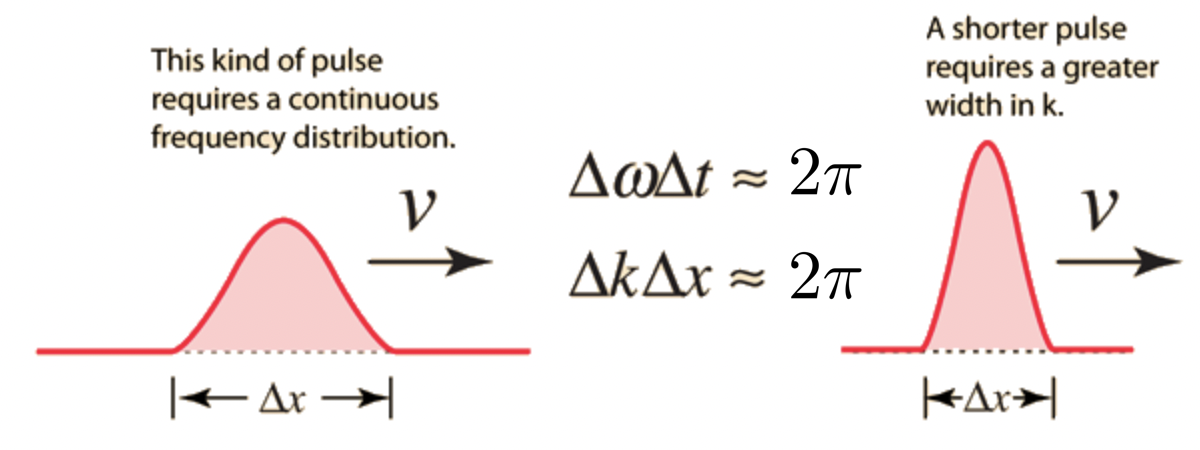
\includegraphics{figs/rel-indet}
    %    \caption{This is a margin figure.}
    \label{fig:rel-indet}
\end{marginfigure}

In generale si può dimostrare che valgono le seguenti relazioni
\begin{gather*}
    \Delta k_{x} \Delta x \simeq2 \pi\\
    \Delta k_{y} \Delta y \simeq2 \pi\\
    \Delta k_{z} \Delta z \simeq2 \pi\\
    \Delta \omega \Delta t \simeq2 \pi
\end{gather*} Nel caso in cui si abbia un pacchetto d'onde che contenga solo una
componente di Fourier si avrebbe
\(\Delta k_{x} = \Delta k_{y} = \Delta k_{z} = 0\) con una conseguente
indeterminazione sulle posizioni tendente a \(\infty\).

Consideriamo il caso di un'onda piana,di lunghezza d'onda \(\lambda\) e
vettore d'onda \(\bm{k} = k_x \hat{\imath}\), che viene fatta passare
attraverso una fenditura ampia \(d\) (vedi Figura~\ref{fig:wave-electron-experiment}).

\begin{marginfigure}
    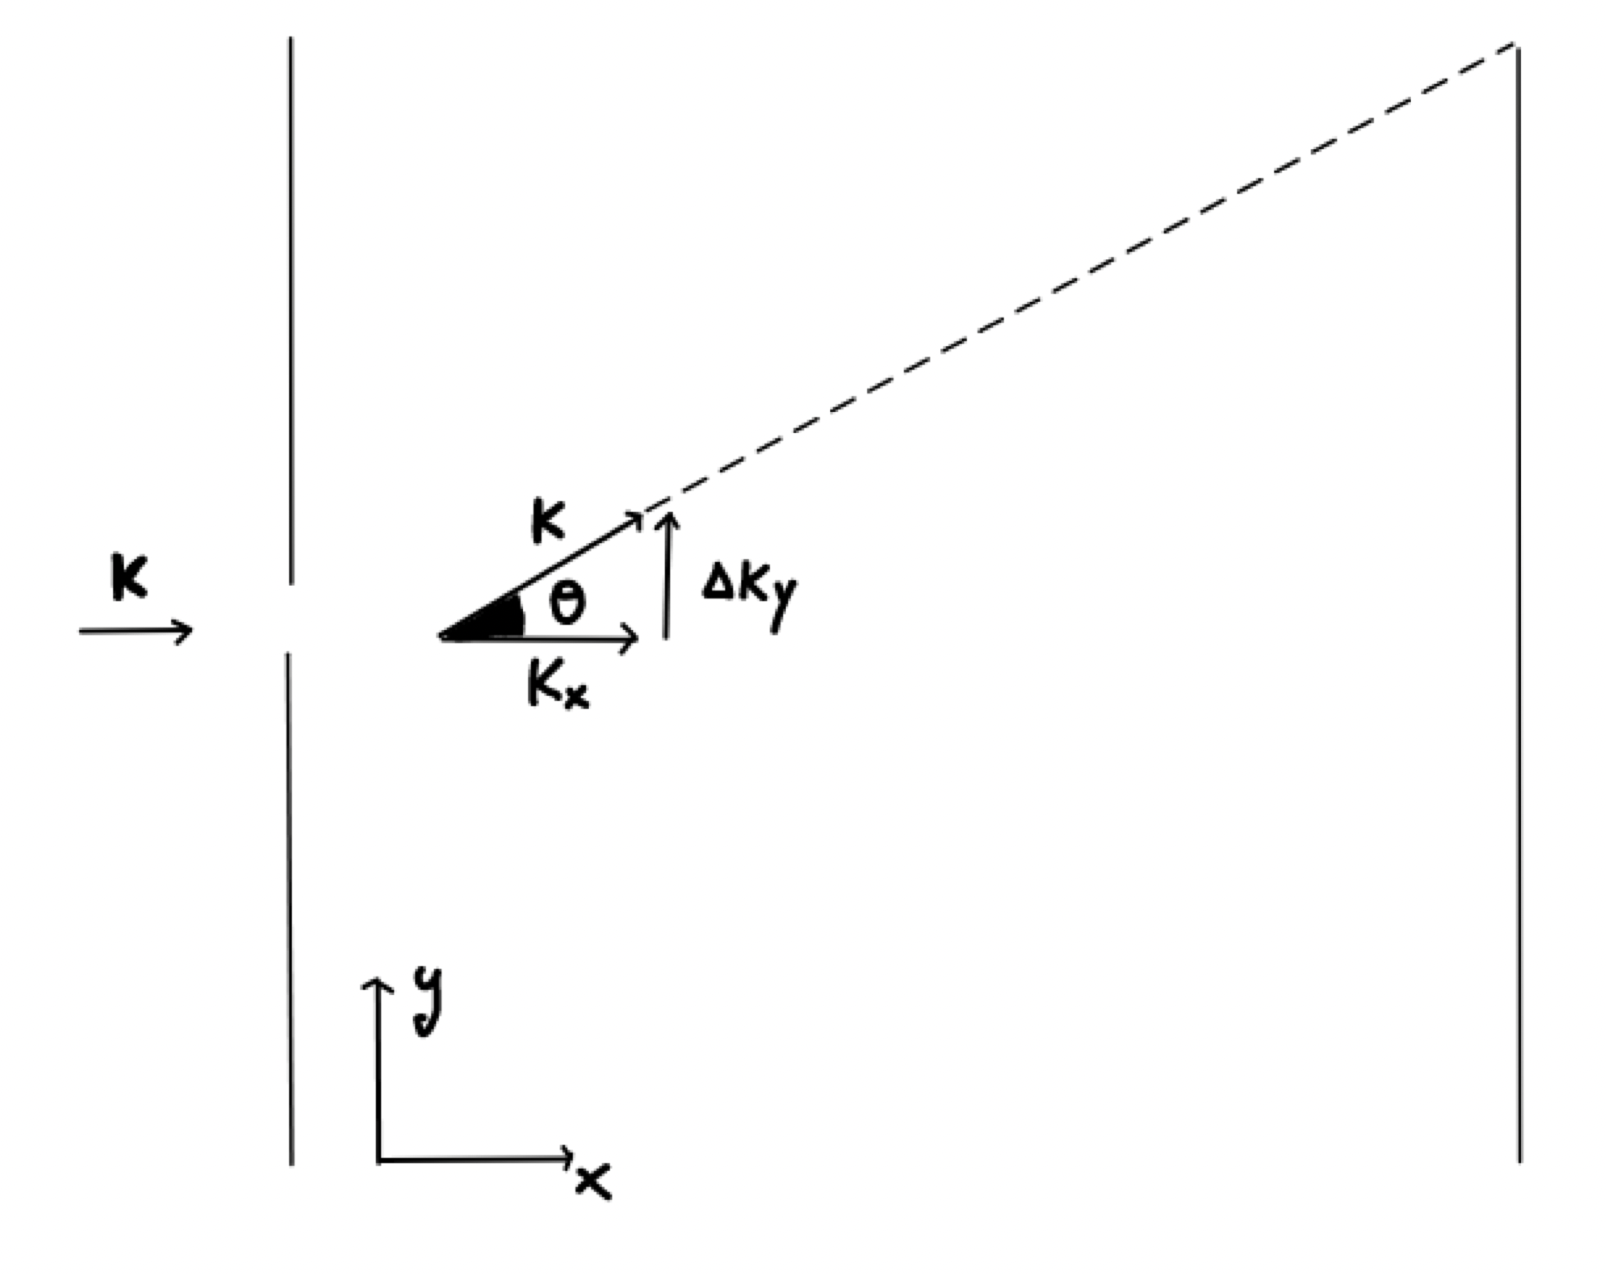
\includegraphics{figs/wave-electron-experiment}
    \caption{Esperienza classica per evidenziare l'effetto dell'indeterminazione.}
    \label{fig:wave-electron-experiment}
\end{marginfigure}

Il fronte d'onda viene tagliato dalla fenditura stessa: il fronte d'onda
lungo \(y\) ha un'incertezza \(\Delta y = d\).
Dalle relazioni
precedenti so che viene introdotto un errore
\(\Delta k_{y} \simeq\frac{2\pi}{d}\) .
La fenditura ha deviato il
vettore d'onda \(\bm{k}\) ed ora ha una certa angolazione \(\implies\)
il fronte d'onda che si incurva (in accordo con il Principio di Huygens-Fresnel).
L'angolo di apertura vale quindi \[
                                     \theta \simeq\frac{\Delta k_{y}}{k_{x}} \simeq \frac{2\pi}{d  \frac{2\pi}{\lambda}} \simeq\frac{\lambda}{d}
\] In ultima analisi quindi il fronte d'onda viene \textbf{limitato
spazialmente} e dà luogo al fenomeno della \textbf{diffrazione}.

Vogliamo ora trovare l'analogo delle relazioni di indeterminazione in
\textbf{meccanica quantistica}.
Partiamo dalle relazioni \[
                             \bm{p} = \hslash \bm{k} \qquad E = \hslash \omega \qquad p_{x} = \hslash k_{x}
\] e arriviamo a
\begin{gather}
    \Delta p_{x} \Delta x \simeq h\\
    \Delta p_{y} \Delta y \simeq h\\
    \Delta p_{z} \Delta z \simeq h\\
    \Delta E \Delta t \simeq h
\end{gather}
relazioni note come \textbf{relazioni di indeterminazione di
Heisenberg} le quali affermano che
\begin{enumerate}
    \tightlist
    \item
    se la misura della posizione di un corpuscolo materiale lungo una
    certa direzione ha una incertezza \(\Delta x\) allora una simultanea
    misura della quantità di moto lungo la stessa direzione ha una
    incertezza \(\Delta p_x\) tale che il loro prodotto sia dell'ordine
    della costante di Plank;
    \item
    se la misura della posizione temporale di un corpuscolo materiale ha
    una incertezza \(\Delta t\) allora una simultanea misura della energia
    ha una incertezza \(\Delta E\) tale che il loro prodotto sia
    dell'ordine della costante di Planck.
\end{enumerate}

Un analogo quantistico dell'esperimento precedente può consistere
nell'inviare un elettrone con quantità di moto
\(\bm{p} = p_{x} \hat{\imath}\) verso una fenditura di ampiezza \(d\).
Nel
momento in l'elettrone passa in mezzo alla fenditura possiamo
sicuramente dire che la sua posizione assume un qualche valore
\emph{all'interno del range} della fenditura (vedi Figura~\ref{fig:beam-electron-experiment}).
Si ha quindi che il passaggio attraverso essa e la conseguente limitazione sulla posizione
della posizione \emph{equivale ad un'operazione di misura} sulla
particella.

\begin{marginfigure}
    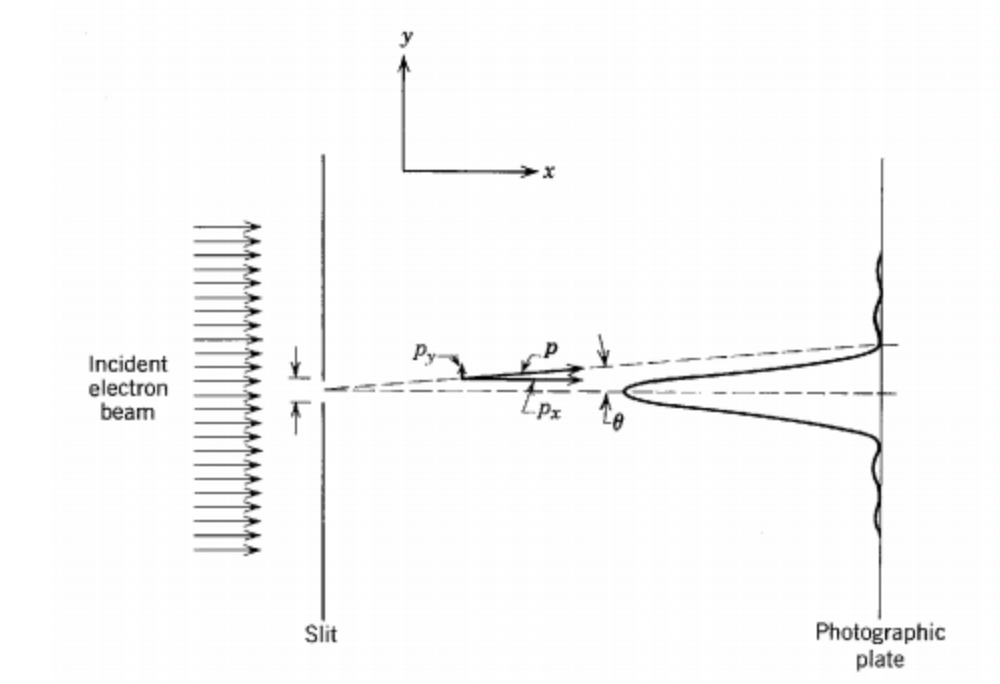
\includegraphics[width = 1.3 \textwidth, height = 1.3 \textheight]{figs/beam-electron-experiment}
    \caption{Esperienza quantistica per evidenziare l'effetto dell'indeterminazione.}
    \label{fig:beam-electron-experiment}
\end{marginfigure}

\[
    \Delta y \simeq d \qquad \Delta p_{y} \simeq \frac{h}{d}
\] con angolo di inclinazione
\[
    \theta \simeq \frac{\Delta p_{y}}{p_{x}} \simeq \frac{h}{d \frac{h}{\lambda}} \simeq \frac{\lambda}{d}
\]
\bigskip

L'incompatibilità tra le variabili dinamiche di un sistema
quantomeccanico è espressa in forma precisa da un fondamentale teorema
della meccanica quantistica il quale stabilisce che

\begin{quote}
    Il prodotto delle deviazioni standard delle misure di due grandezze
    fisiche \(a\) e \(b\) in uno stato \(\psi\) è limitato inferiormente dal
    valore di aspettazione del commutatore dei loro operatori diviso il
    fattore \(2i\)
    \begin{equation}
        \boxed{\sigma_{a} \sigma_{b} \geq \iiint_{V} \bar{\psi}(\bm{r},t) \frac{\hat{A}\hat{B} -\hat{B}\hat{A}}{2i}
        \psi(\bm{r},t) \, dV}
        \label{eq:sigma-product-commutator-theorem}
    \end{equation}
\end{quote}

A titolo di esempio possiamo considerare proprio le variabili dinamiche
di posizione e quantità di moto
\[
    a = p_x \qquad b = x
\]
con corrispondente operatori \[
                                 - i \hslash \frac{\partial}{\partial x} \qquad x
\] e calcolarne il commutatore
\[
    \hat{X}\hat{P}_{x} - \hat{P}_{x}\hat{X}
\] per cui calcoliamo i due termini \begin{gather*}
                                        \hat{X}\hat{P}_{x} \psi = x \left(  - i \hslash \frac{\partial}{\partial x} \right) \psi = - i \hslash x \frac{\partial}{\partial x}\psi\\
                                        \hat{P}_{x}(\hat{X} \psi) = \left( - i \hslash \frac{\partial}{\partial x} \right)(x \psi)  =
                                        - i \hslash \left( \psi - x \frac{\partial}{\partial x} \psi \right) = - i \hslash \psi - i \hslash x \frac{\partial}{\partial x} \psi
\end{gather*}
ed otteniamo
\[
    (\hat{X}\hat{P}_{x} - \hat{P}_{x}\hat{X}) \psi = - i \hslash x \frac{\partial}{\partial x}\psi - \left[ - i \hslash \psi - i \hslash x \frac{\partial}{\partial x} \psi \right] = i \hslash \psi
\]
da cui il valore del commutatore
\[
    \hat{X}\hat{P}_{x} - \hat{P}_{x}\hat{X} = i \hslash  \hat{1}
\]
che sostituito nella (\ref{eq:sigma-product-commutator-theorem}) fornisce
\begin{gather*}
    \sigma_{x} \sigma_{p_{x}} \geq \iiint_{V} \bar{\psi}(\bm{r},t) \frac{\hat{X}\hat{P}_{x} - \hat{P}_{x}\hat{X}}{2 i } \psi(\bm{r},t) \, dV =
    \iiint_{V} \bar{\psi}(\bm{r},t) \frac{i \hslash  \hat{1}}{2i}\psi(\bm{r},t) \, dV\\
    \sigma_{x}\sigma_{p_{x}} \geq \frac{\hslash}{2}
\end{gather*}
che esprime in forma rigorosa il principio di indeterminazione per le
misure della posizione e quantità di moto.

\section{Momento angolare orbitale}\label{sec:momento-angolare-orbitale}

Il momento angolare orbitale è un ottimo esempio per comprendere come si
possa utilizzare il \emph{principio di corrispondenza} per costruire
l'operatore quantomeccanico di una variabile dinamica a partire dalla
sua espressione classica
\[
    \bm{l}  = \bm{r} \wedge \bm{p}
\]
L'idea è quella di ottenere l'espressione quantomeccanica
dell'operatore associato attraverso la sostituzione diretta delle
variabili classiche con i corrispondenti operatori quantistici.
Richiamando allora gli operatori posizione e quantità di moto, otteniamo
la seguente espressione della terna ordinata di operatori che
costituiscono \textbf{l'operatore momento della quantità di moto}
\begin{equation}
    \hat{L} = \hat{r} \wedge \hat{P}=\bm{r} \wedge (- i \hslash \nabla) = - i \hslash \ \bm{r} \wedge \nabla
    \label{eq:momentum-operator-2}
\end{equation}
la quale, nel sistema di coordinate cartesiano, assume la seguente forma
\begin{equation}
    \hat{L} = (\hat{L}_{x}, \hat{L}_{y}, \hat{L}_{z}) = - i \hslash \left( y \frac{\partial}{\partial z} - z \frac{\partial}{\partial y},z \frac{\partial}{\partial x}-x \frac{\partial}{\partial z}, x \frac{\partial}{\partial y} - y \frac{\partial}{\partial x} \right)
    \label{eq:momentum-operator-cartesian-coordinates}
\end{equation}
Dato che le proprietà generali di un operatore possono essere
studiate attraverso le sue relazioni di commutazione, utilizziamo la
foma cartesiana esplicita per calcolare i commutari della terna di
operatori.
Si ottiene facilmente
\begin{equation}
    [\hat{L}_{x},\hat{L}_{y}] = i \hslash  \hat{L}_{z} \quad
    [\hat{L}_{z},\hat{L}_{x}] = i \hslash  \hat{L}_{y} \quad
    [\hat{L}_{y},\hat{L}_{z}] = i \hslash  \hat{L}_{x}
    \label{eq:commutators-momentum-operator}
\end{equation}
Verifichiamo allora che uno stato quantomeccanico non ammette valori
definiti del momento della quantità di moto lungo \(x, y\) e \(z\)
poiché la proiezione lungo \(x\) è incompatibile con quella lungo \(y\),
quella lungo z con quella lungo \(x\) e quella lungo \(y\) con quella
lungo \(z\).
\begin{marginfigure}
    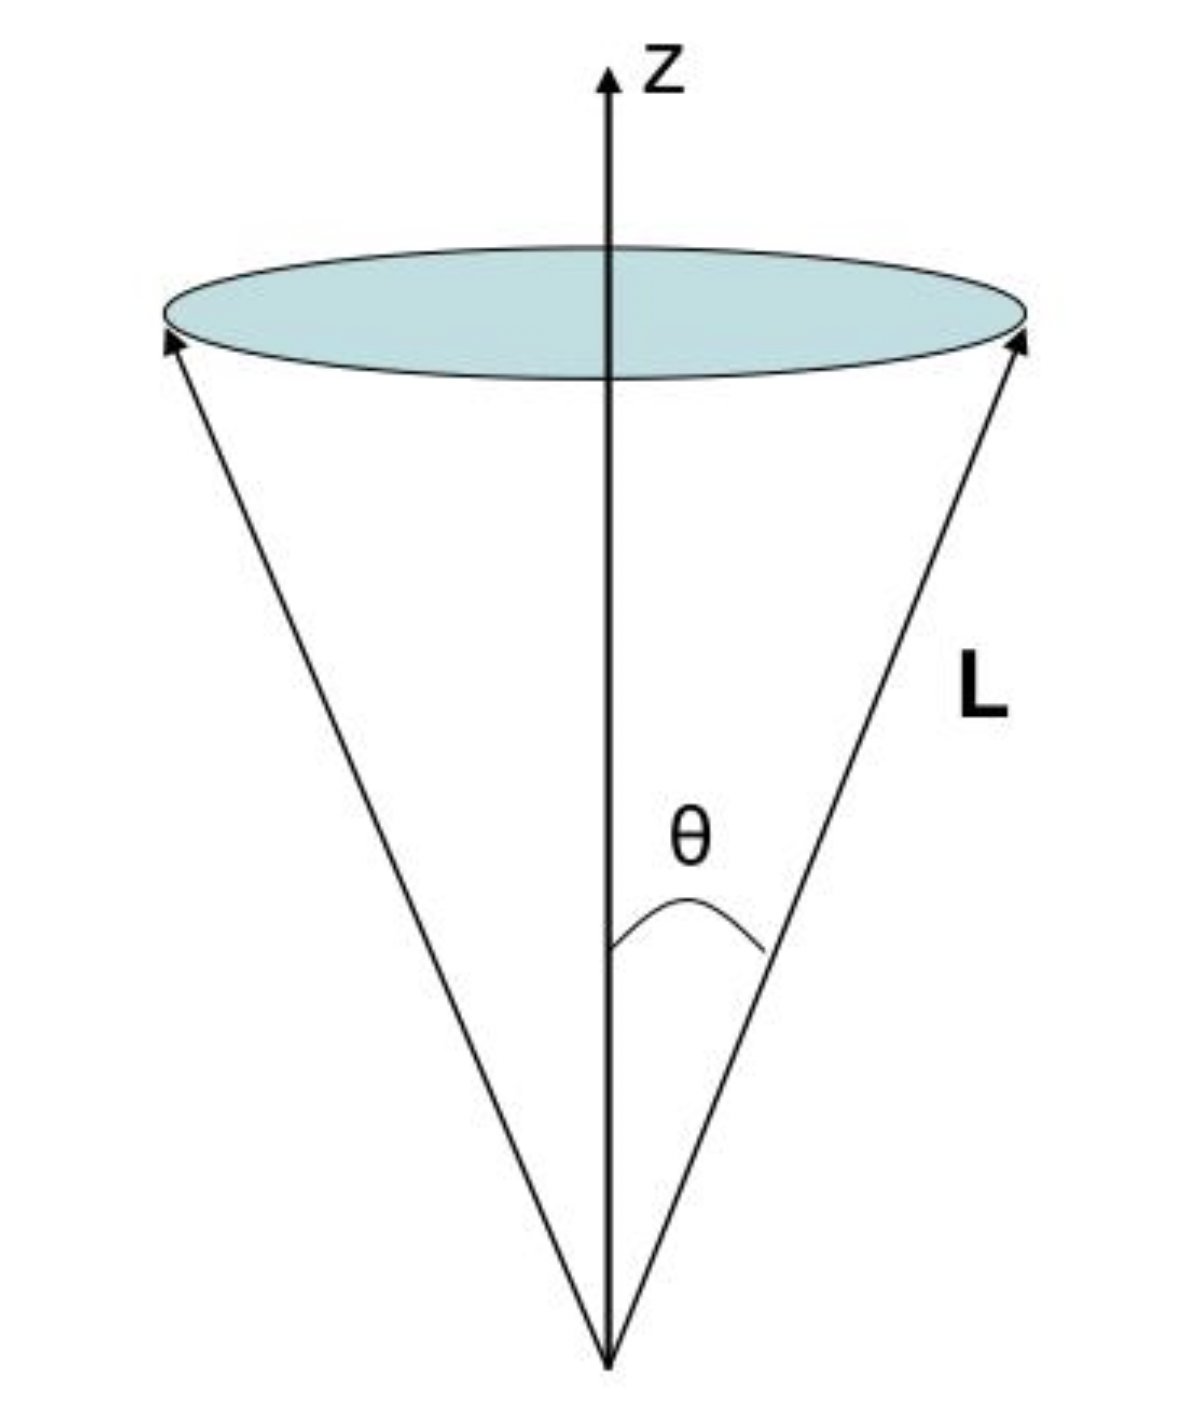
\includegraphics{figs/ang-mom-cone}
    \caption{Il set dei possibili valori di $\hat{L_x}$ e $\hat{L_y}$ descrive un cono attorno ad $\hat{L}_z$}
    \label{fig:ang-mom-cone}
\end{marginfigure}
Ciò significa che \emph{in uno stato quantomeccanico il
momento angolare può assumere valori definiti lungo una sola direzione}
che solitamente si assume come asse \(z\).
Consideriamo ora l'operatore \textbf{modulo quadrato del momento
angolare}
\begin{equation}
    \hat{L}^{2} = \hat{L}_{x}^{2} + \hat{L}_{y}^{2} + \hat{L}_{z}^{2}
    \label{eq:square-modulus-momentum-operator}
\end{equation} Sempre con calcolo diretto si ottengono facilmente i seguenti
commutatori
\begin{equation}
    \left[ \hat{L}^{2},\hat{L}_{x}\right] = \left[ \hat{L}^{2},\hat{L}_{y}\right] = \left[ \hat{L}^{2},\hat{L}_{z}\right] = 0
    \label{eq:commutators-square-modulus-momentum-operator}
\end{equation}
Dalle relazioni di commutazioni (\ref{eq:commutators-momentum-operator}) e (\ref{eq:commutators-square-modulus-momentum-operator}),
concludiamo allora che
\textbf{uno stato quantomeccanico ammette valori definiti del quadrato
del momento angolare e della sua componente lungo \(z\)} (vedi Figura~\ref{fig:ang-mom-cone}).
\bigskip

Giunti a questo punto si pone il problema di stabilire quali siano i
valori definiti del quadrato del momento angolare e della sua componente
lungo z e quali siano le espressioni della funzione d'onda dei
corrispondenti stati quantomeccanici.
Per rispondere a queste domande
occorre risolvere le equazioni agli autovalori degli operatori.
In
particolare, gli \textbf{autovalori forniranno i possibili valori del
quadrato del momento angolare e della sua terza componente}, mentre le
corrispondenti \textbf{autofunzioni} forniranno le espressioni delle
\textbf{funzioni d'onda} degli stati quantomeccanici: \begin{gather*}
                                                          \hat{L}^{2}\psi = \lambda \psi\\
                                                          \langle \hat{L}^{2}\rangle = \iiint_{V} \bar{\psi} \hat{L}^{2}\psi \, dV = \lambda \iiint_{V} \psi \bar{\psi} \, dV = \lambda\\
                                                          \hat{L}^{2} \psi = \lambda' \psi \qquad  \hat{L}_{z} \psi = \lambda'' \psi
\end{gather*}
Sviluppando il conto (vedi un testo di QM) si ha
\begin{align*}
    \hat{L}^{2}\psi_{l,m} &= l(l+1) \hslash^{2} \psi_{l,m} \qquad  \, l = 0,1,2, \dots , n\\
    \hat{L}_{z} \psi_{l,m} &= m \hslash \psi_{l,m} \qquad  \qquad \quad \, m = -l,-l + 1, \dots ,l-1, l
\end{align*} Siamo difronte ad un operatore \textbf{quantizzato} ovvero che può
assumere valori \textbf{discreti}: i numeri interi $l$ ed $m$ descrivono
compiutamente lo stato quantomeccanico e vengono detti numeri quantici
del momento angolare.\\
\begin{marginfigure}
    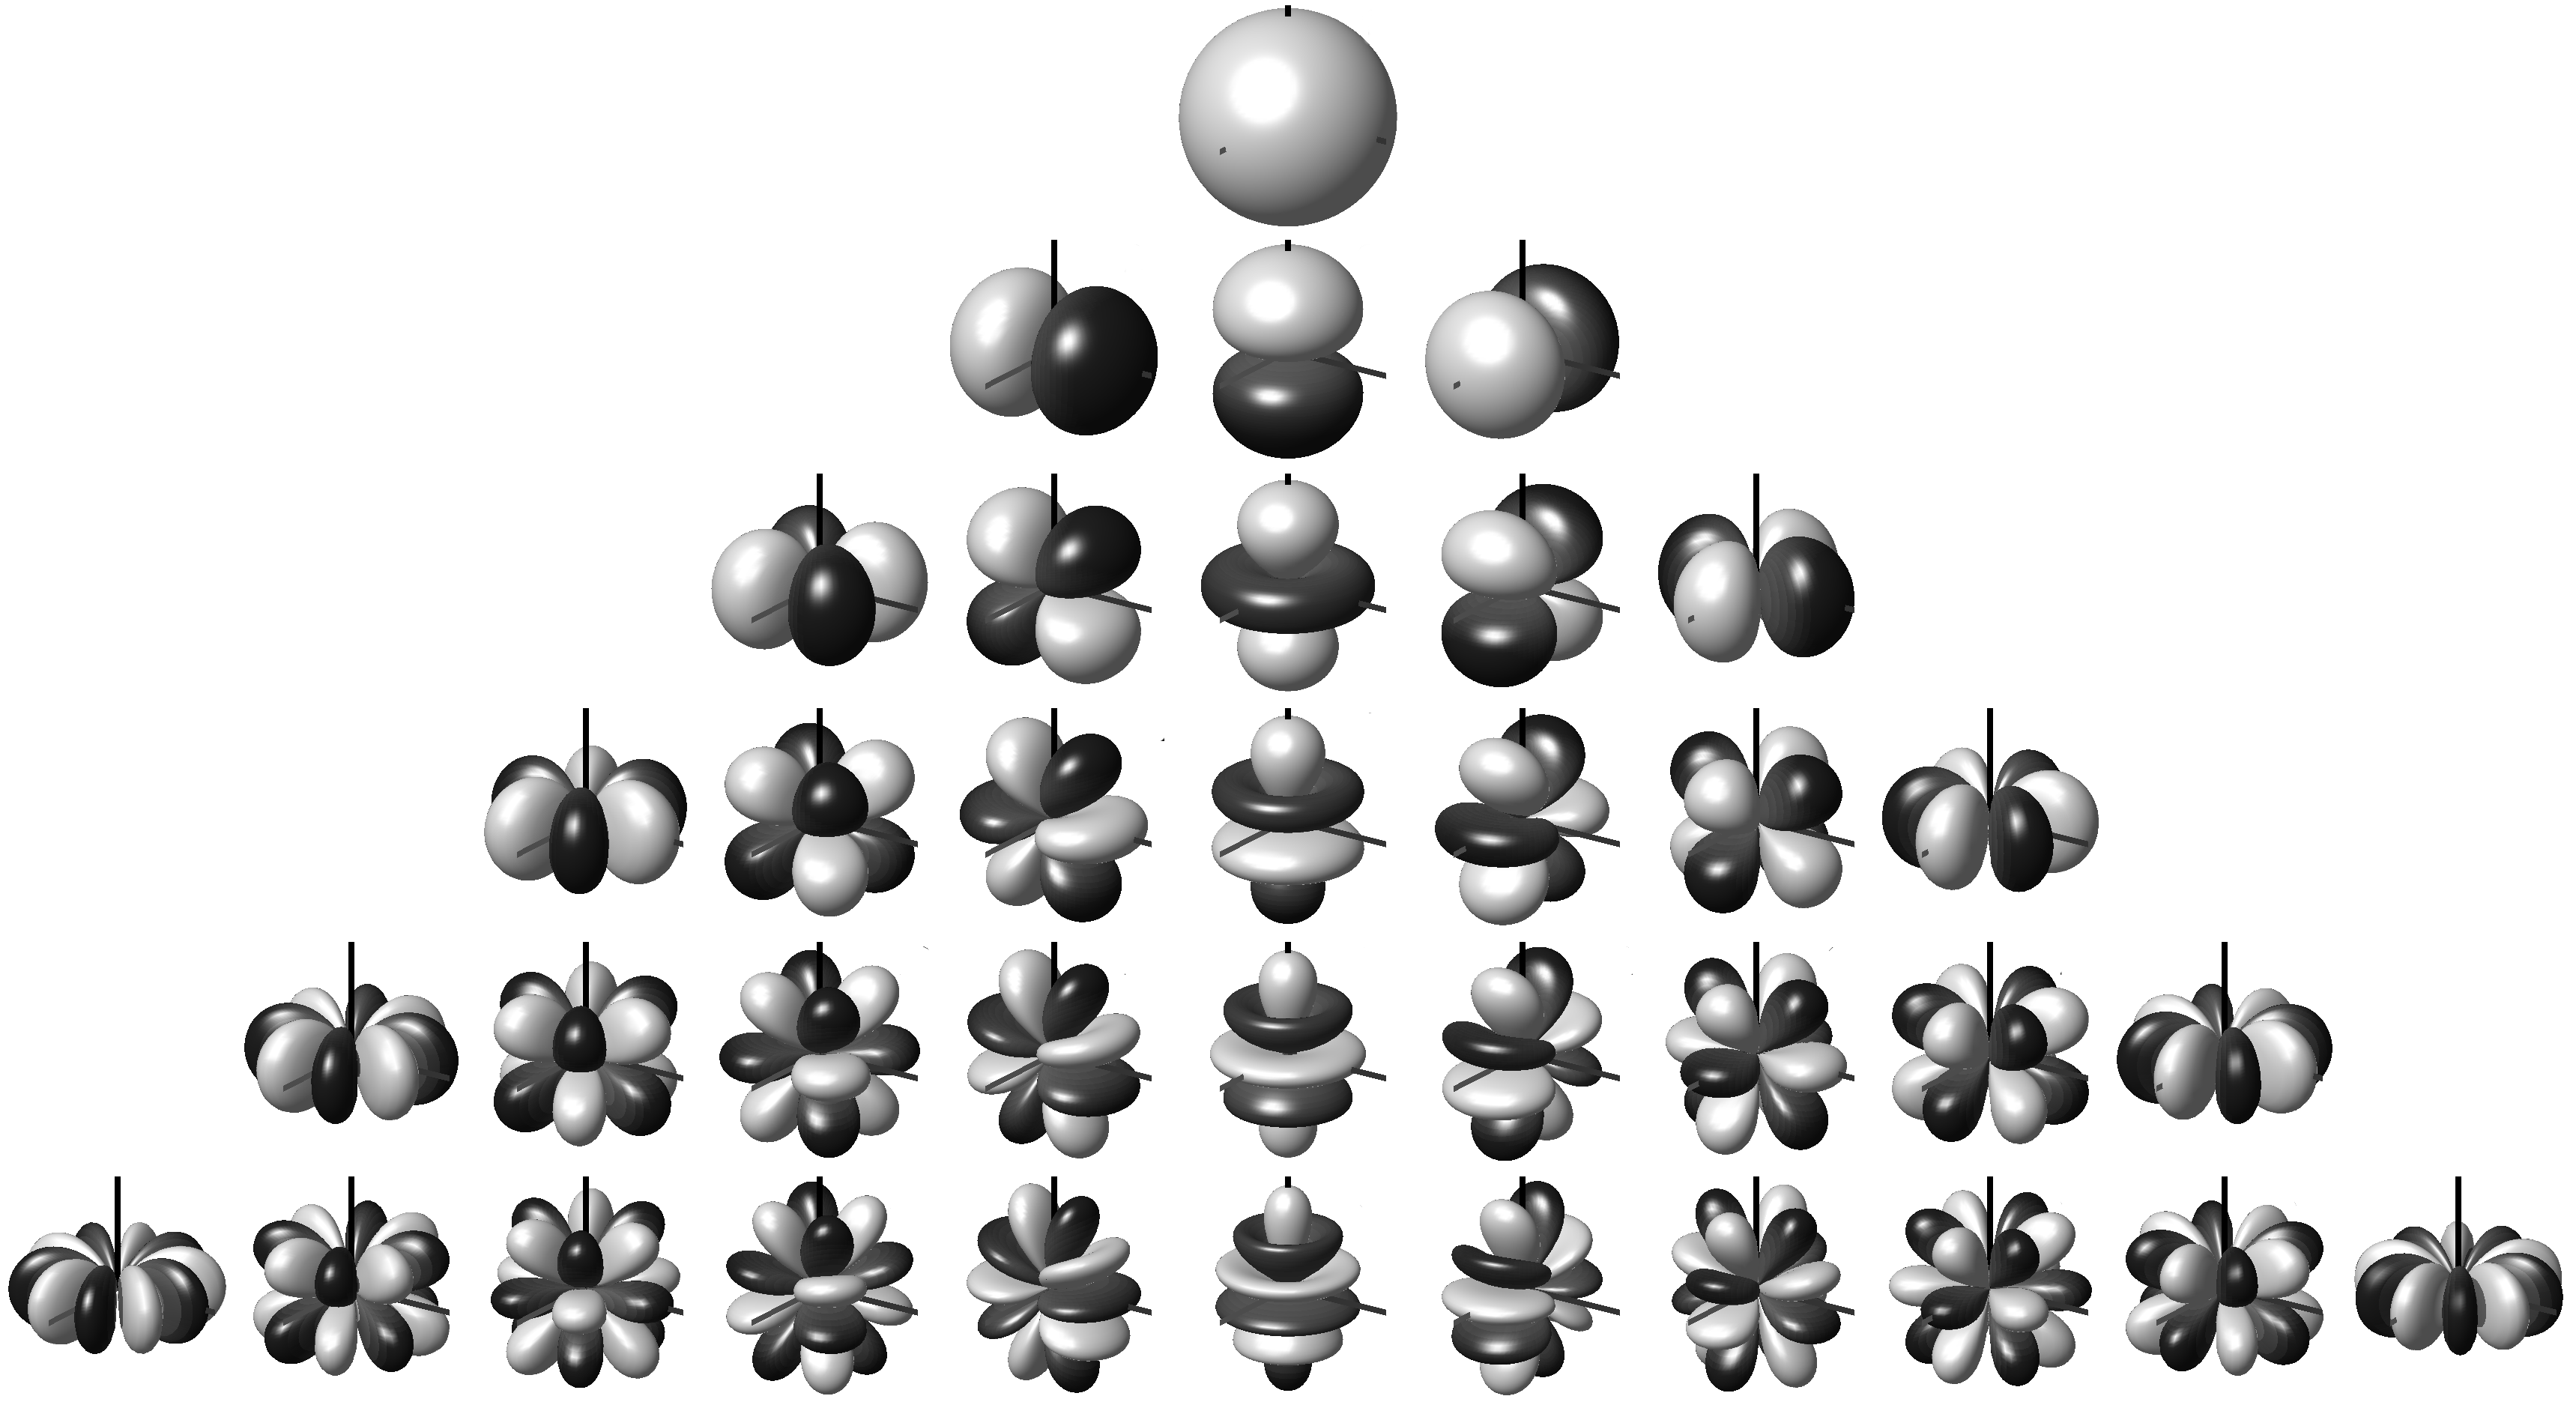
\includegraphics{figs/spherical-harmonics}
    \caption{Rappresentazione grafica delle prime armoniche sferiche.}
    \label{fig:spherical-harmonics}
\end{marginfigure}
In particolare le coppie di valori l ed m individuano spefiche funzioni
d'onda \(\psi_{l,m}(\theta,\phi)\) dette \textbf{armoniche sferiche}.
This peculiar set of functions comes out in the classical theory as well
when considering the modes of oscillation of a 2-dimensional membrane.
\marginnote
{
   \begin{gather*}
            l = 0 \quad m = 0 \\
                  l(l+1) \hslash^2 = m \hslash = 0 \\
                  Y_{0,0}(\theta,\phi) \\ \\
                  l = 1 \quad m = -1,0,1 \\
                  l(l+1) \hslash^2 = 2 \hslash^2 \quad m \hslash = - \hslash,0, \hslash \\
                  Y_{1,-1}(\theta,\phi) \quad Y_{1,0}(\theta,\phi) \quad Y_{1,1}(\theta,\phi) \\ \\
                        l = 2 \quad m = -2,-1,0,1,2 \\
                        l(l+1) \hslash^2 = 6 \hslash^2 \quad m \hslash = -2 \hslash, - \hslash,0,\hslash,2 \hslash
        \end{gather*}
}
I possibili valori del quadrato del momento angolare sono dati dalla
successione discreta \(l(l+1) \hslash^{2}\) dove \(l=0,1,2 \dots\)
mentre i possibili valori del momento angolare lungo z sono dati dalla
successione discreta \(m \hslash\) dove
\(m = -l, -l + 1, \dots, l-1, l\) ovvero da una sequenza di \(2l+1\)
valori interi dipendente da \(l\).

\section{Momento angolare intrinseco o spin}\label{sec:momento-angolare-intrinseco-o-spin}

Lo spin delle particelle microscopiche è un esempio di variabile dinamica che, pur suggerita da inesatte analogie con
la fisica classica, risulta essere di fatto una grandezza fisica di natura esclusivamente quantomeccanica.

Nella meccanica classica i corpi materiali puntiformi possiedono al più
solo momento angolare orbitale mentre quelli estesi possono essere
portatori anche di un momento angolare intrinseco (spin).
Scegliendo il
polo di riduzione coincidente con il centro di massa del corpo
materiale, il momento angolare orbitale si annulla e l'unico momento
angolare residuo del corpo esteso è quello intrinseco che si manifesta
come rotazione del corpo stesso attorno ad un asse baricentrico.

Date queste premesse, ci si può domandare se anche le particelle
microscopiche possiedano un momento angolare intrinseco (spin) in
aggiunta al momento angolare orbitale.
I fatti sperimentali mostrano che
la risposta è affermativa e che il momento angolare intrinseco o spin
deve essere introdotto anche nel caso delle particelle microscopiche.
Vi
sono però delle sostanziali differenze

\begin{itemize}
    \tightlist
    \item
    \textbf{meccanica classica}: un momento angolare intrinseco o residuo
    può esistere solo per i \emph{corpi estesi} (non puntiformi) e questo
    si interpreta come la somma dei momenti angolari orbitali di tutte le
    parti che lo compongono;
    \item
    \textbf{meccanica quantistica}: un momento angolare intrinseco o di
    spin può esistere anche per le particelle puntiformi e come tale non è
    riducibile in nessun modo a somme di momenti angolari orbitali delle
    parti del sistema;
    \item
    \textbf{meccanica classica}: il modulo del momento angolare intrinseco
    può assumere con \emph{continuità qualunque valore}, ha un carattere
    estrinseco e descrive essenzialmente lo stato cinematico di rotazione
    del sistema rispetto ad un prefissato riferimento;
    \item
    \textbf{meccanica quantistica}: il modulo del momento angolare
    intrinseco può assumere un solo valore \emph{fisso} ed
    \emph{immutabile}.
    A seguito di tale invariabilità perde il suo
    carattere estrinseco di natura cinematica ed assume - al pari della
    massa e delle cariche interne del corpuscolo - lo status di grandezza
    fisica intrinseca preposta alla descrizione di una nuova proprietà
    statica della particella.
\end{itemize}

Per questi ed altri motivi possiamo affermare che \emph{lo spin è una
variabile dinamica essenziamente quantistica} senza una diretta
corrispondenza classica.

Pauli pensò che fosse necessario introdurre una \textbf{terna di
operatori di spin} \[
                       S_{x} \qquad S_{y} \qquad S_{z}
\] soddisfacenti le regole di commutazione `tipo momento angolare'
\begin{equation}
[ S_{x},S_{y}] = i \hslash S_{z} \qquad  [ S_{y},S_{z}] = i \hslash S_{x} \qquad   [ S_{z},S_{x}] = i \hslash S_{y}
\label{eq:commutators-spin-operator}
\end{equation}
ed operano sullo \textbf{spazio degli stati di spin}, uno `spazio
interno' diverso da quello su cui operano gli operatori del momento
angolare orbitale (lo spin è dunque un nuovo grado di libertà del
sistema microscopico).

In analogia con il caso del momento della quantità di moto, le regole di
commutazione (\ref{eq:commutators-spin-operator}) implicano che \textbf{uno stato
quantomeccanico ammette valori definiti del modulo quadrato dello spin e
della sua terza componente}.

In particolare, risolta l'equazione agli autovalori degli operatori
quadrato del momento angolare di spin e della sua terza componente si
può ottenere l'insieme degli autovalori e delle autofunzioni (si veda un testo di QM):
\begin{equation}
    \begin{aligned}
        \hat{S}^{2} \eta_{s,s_{z}} &= s (s+1) \hslash^{2} \eta_{s,s_{z}} \qquad s = 0, \frac{1}{2}, 1, \frac{3}{2}, \dots \\
        \hat{S}_{z} \eta_{s,s_{z}} &= s_{z} \hslash \eta_{s,s_{z}} \qquad \qquad \quad s_{z} = -s, -s+1, \dots , s-1, s
    \end{aligned}
    \label{eq:eigenvalue-eq-spin}
\end{equation}

dove \(s_{z}\) compie salti unitari tra un valore di \(s\) e il
seguente.
I numeri interi e/o seminteri $s$ e $s_{z}$ descrivono compiutamente lo stato quantomeccanico di spin e vengono detti \textbf{numeri quantici delo spin}.
Essi permettono di calcolare i possibili valori dello spin (autovalori) ed individuano i corrispondenti \emph{vettori di stato} $\eta_{s,s_{z}}$ \\
Ad esempio:
\begin{itemize}
    \item Se $s = 0,s_{z}=0$ si ha $s(s+1) \hbar^{2} = 0 \ , \ s_{z}\hbar = 0$ con vettore di stato $\eta_{0,0}$ (in tal caso si dice che la particella non ha spin);
    \item Se $s=\frac{1}{2}, s_{z} = -\frac{1}{2}, \frac{1}{2}$ si ha $s(s+1)\hbar = \frac{3}{4} \hbar^{2} \ , \ s_{z}\hbar = -\frac{1}{2}\hbar, \frac{1}{2} \hbar$ con vettori di stato $\eta_{\frac{1}{2} , - \frac{1}{2}} , \eta_{\frac{1}{2}, \frac{1}{2}}$;
    \item Se $s=1 , s_{z} = -1,0,1$ si ha $s(s+1)\hbar = 6\hbar^{2} \ , \ s_{z}\hbar = - \hbar,0, +\hbar$ con vettori di stato $\eta_{1,-1}, \eta_{1,0},\eta_{1,1}$.
\end{itemize}
Si verifica così che, fissato il numero quantico di spin s, lo spazio interno degli stati di spin possiede
$2s+1$ \emph{vettori di stato} $\eta_{s},\eta_{s_{z}}$ linearmente indipendenti ed eventualmente normalizzati per cui deduciamo che \textbf{lo spazio degli stati di spin corrispondente al numero quantico  è uno ‘spazio interno’ complesso di 2s+1 dimensioni}.
\bigskip

Da quanto detto consegue che lo stato quantomeccanico di una particella microscopica di spin $s$ dovrà essere rappresentato nello \emph{spazio prodotto} dello \emph{spazio degli stati quantomeccanici 'ordinari’} già visto, con lo \emph{spazio degli stati di spin}, ovvero dalla funzione d’onda ‘estesa’ o \emph{vettore di stato}
\[
\xi(\mathbf{r},t) = \psi(\mathbf{r},t) \eta_{s,s_{z}}
\]
\begin{marginfigure}
    L'analogo classico piu vicino all'onda piana, con
    \(\eta_{\frac{1}{2}, \frac{1}{2}}\) ampiezza spinoriale,
    \[
        \eta_{\frac{1}{2}, \frac{1}{2}} \psi_{0}e^{ i/\hslash (\bm{p}\cdot \bm{r} - Et)}
    \] è un'onda piana di campo elettrico
    \[
        \bm{E}_{0} \sin(\bm{k}\cdot \bm{r} - \omega t) \, \cdot
    \]
\end{marginfigure}
Premesso che nel caso di spin $s=0$ la funzione d’onda ‘estesa’ si riduce alla ordinaria funzione d’onda, il caso immediatamente seguente è quello dello spin $s=1 / 2$ cui corrispondono due ‘versori’ indipendenti $\eta_{\frac{1}{2}, \frac{1}{2}}$ e $\eta_{\frac{1}{2}, - \frac{1}{2}}$ e dunque uno spazio degli stati di spin a due dimensioni. I costituenti dell’atomo, ovvero gli elettroni i neutroni ed i protoni, hanno \emph{spin} $s=1/2$ sono pertanto descritti da vettori di stato del tipo seguente
\[
\psi(\mathbf{r},t) \eta_{\frac{1}{2}, - \frac{1}{2}} \qquad \psi(\mathbf{r},t) \eta_{\frac{1}{2}, \frac{1}{2}}
\]

Usando una terminologia diffusa, il primo potrebbe descrivere un protone nello stato $\Psi$ con spin ‘giu’ ed il secondo un protone nello stato $\Psi$ con spin ‘su’.
\bigskip

E’ importante sottolineare che l’introduzione di uno ‘spazio interno complesso’ per la descrizione degli stati di spin delle particelle microscopiche costituisce un precedente teorico di grande rilevanza.
Infatti essa suggerisce che eventuali \emph{gradi di libertà interni} delle particelle microscopiche richiesti dai dati sperimentali possano essere descritti in ambito quantomeccanico semplicemente introducendo opportuni \emph{spazi vettoriali complessi} dotati della giusta dimensionalità.

La fisica delle particelle sfrutterà a fondo questa possibilità, ma già la fisica nucleare se ne servì sin dai suoi esordi.
Infatti, pochi anni dopo l’introduzione dello spin da parte di W. Pauli nel 1924 (va detto con successivi contributi da parte di Kronig, Uhlenbeck e Goudsmith), Heisenberg (1932) introdusse uno ‘spazio complesso interno’ dove protone e neutrone erano pensati come stati differenti di una unica particella, il nucleone.
Una idea rivoluzionaria che poggiava sul fatto sperimentale che le loro masse erano molto prossime e che per quanto riguarda le interazioni forti neutrone e protone erano sostanzialmente intercambiabili.
Nel 1937, Wigner fornirà la formulazione generale di tale idea introducendo lo \emph{spazio di isospin}, progenitore di tutti gli spazi complessi interni di cui si servirà la fisica delle particelle.
\bigskip

\emph{Esempio - Spazio di spinori 2 dimensionale}.
Fino ad ora gli operatori dello spin sono stati indicati in modo simbolico, essenzialmente definiti dalle leggi di
commutazione (\ref{eq:commutators-spin-operator}) e dalle equazioni agli autovalori (\ref{eq:eigenvalue-eq-spin}).
Nel caso dello spin $s=1/2$ vogliamo dare a questi operatori un’espressione matriciale.
Consideriamo uno spazio di spinori identificato da \[
                                                       s = \frac{1}{2} \qquad s_{z} = - \frac{1}{2} , \frac{1}{2}
\] per cui si hanno gli spinori \[
                                    \xi_{\frac{1}{2}, \frac{1}{2}} \qquad \xi_{- \frac{1}{2}, \frac{1}{2}}
\] Per quanto riguarda gli operatori di spin si ha \[
                                                       \hat{S}^{2} \xi_{\frac{1}{2}, \pm \frac{1}{2}} = \frac{3}{4} \hslash^{2} \xi_{\frac{1}{2}, \pm \frac{1}{2}}
\] e \[
         \hat{S}_{z} \xi_{\frac{1}{2}, \frac{1}{2}} = \frac{1}{2} \hslash \xi_{\frac{1}{2}, \frac{1}{2}} \qquad
         \hat{S}_{z} \xi_{\frac{1}{2}, - \frac{1}{2}} = - \frac{1}{2} \hslash \xi_{\frac{1}{2}, -\frac{1}{2}}
\] Lo spazio è chiaramente bidimensionale dove le direzioni sono
identificate dai 2 spinori.
Nel momento in cui si utilizza uno spazio astratto per rappresentare lo
spin è necessario che valga la condizione della sovrapposizione di stati
che giustifica la spazializzazione dello spin.
A livello classico tale
richiesta in uno spazio ordinario sarebbe quella che tutte le posizioni
intermedie fossero accessibili.

In ogni caso siamo interessati solamente agli stati normalizzati, e
dunque non è fondamentale operare in tutto lo spazio, bensì possiamo
restringerci alla sfera unitaria.
Per dare una forma piu semplice e concreta agli spinori, eseguiamo la
seguente identificazione
\marginnote{Scegliamo gli autovettori di $ S_z$ normalizzati, ortogonali e giacenti sugli assi.}
\[
                             \xi_{\frac{1}{2}, \frac{1}{2}} =
                             \begin{pmatrix}
                                 1 \\ 0
                             \end{pmatrix} \qquad
                             \xi_{\frac{1}{2}, - \frac{1}{2}} =
                             \begin{pmatrix}
                                 0 \\ 1
                             \end{pmatrix}
\] Gli operatori \(\hat{S}\) assumeranno forma matriciale in tale
rappresentazione \[
                     S_{x,y,z} =
                     \begin{pmatrix}
                         \alpha & \alpha \\
                         \alpha & \alpha
                     \end{pmatrix}
\] Dovendo rispettare la condizione che \(S\) sia \emph{autoaggiunta} la
costruiamo come \[
                    S_{x,y,z} =
                    \begin{pmatrix}
                        a      & b - ic \\
                        b + ic & d
                    \end{pmatrix}
\] Volendo però stare in totale generalità scriveremo
\begin{align*}
    S & =
    \begin{pmatrix}
        a + d & b-ic \\
        b+ic  & a-d
    \end{pmatrix} \\
    & =
    a
    \begin{pmatrix}
        1 & 0 \\
        0 & 1
    \end{pmatrix}
    + b \begin{pmatrix}
            0 & 1 \\
            1 & 0
    \end{pmatrix}
    + c \begin{pmatrix}
            0 & -1 \\
            1 & 0
    \end{pmatrix}
    +d \begin{pmatrix}
           1 & 0  \\
           0 & -1
    \end{pmatrix}
\end{align*}

Notiamo che qualunque matrice è combinazione lineare di queste 4
matrici
\[
    M = a \ I_{2 \times 2} + b \sigma_{1} + c \sigma_{2} + d \sigma_{3}
\]
Tali matrici di base sono la matrice identità e le cosiddette \textbf{matrici di Pauli}.
Osserviamo che la matrice identità non puo far parte in questa base,
altrimenti si andrebbe a perdere la condizione di non commutazione
propria degli operatori di spin (essa commuta con tutte le matrici).
La
rappresentazione matriciale di \(\hat{S}_{z}\) sarà la seguente \[
                                                                    \hat{S}_{z} \begin{pmatrix}
                                                                                    1 \\
                                                                                    0
                                                                    \end{pmatrix} =
                                                                    \frac{1}{2} \hslash \ I
                                                                    \begin{pmatrix}
                                                                        1 \\
                                                                        0
                                                                    \end{pmatrix}
                                                                    \qquad
                                                                    \hat{S}_{z} \begin{pmatrix}
                                                                                    0 \\
                                                                                    1
                                                                    \end{pmatrix}
                                                                    = - \frac{1}{2} \hslash I \begin{pmatrix}
                                                                                                  0 \\
                                                                                                  1
                                                                    \end{pmatrix}
\] \[
       \implies
       \hat{S}_{z} =
       \begin{pmatrix}
           \frac{1}{2} \hslash & 0                     \\
           0                   & - \frac{1}{2} \hslash
       \end{pmatrix}
\] Quindi \(\hat{S}_{z}\) deve essere \textbf{diagonale con i valori di
spin sulla diagonale}.
Quindi quella appena scritta e una base
ortonormale (essendo gia i vettori normalizzati) di \(\hat{S}_{z}\)
\[
    \hat{S}_{z} = \frac{\hslash}{2}
    \begin{pmatrix}
        1 & 0  \\
        0 & -1
    \end{pmatrix} = \frac{\hslash}{2} \sigma_{3}
\] Svolgendo il conto vediamo che anche la relazione di commutazione
\[
    [ \hat{S}_{z}, \hat{S}_{x}] = i \hslash \hat{S}_{y}
\]
è rispettata.
In conclusione
\[
    \hat{S}_{x} = \frac{\hslash}{2} \sigma_{1} \qquad
    \hat{S}_{y} =  \frac{\hslash}{2} \sigma_{2} \qquad
    \hat{S}_{z} = \frac{\hslash}{2} \sigma_{3}
\] Un vettore generico di spin generico si scrive come
\[
    \psi = \psi (\bm{r},t)
    \begin{pmatrix}
        \alpha \\
        \beta
    \end{pmatrix}
\]
Scelta una base ortonormale verifichiamo che
\[
    \hat{S}^{2}
    \begin{pmatrix}
        1 \\
        0
    \end{pmatrix}
    = (\hat{S}_{x}^{2} + \hat{S}_{y}^{2}+\hat{S}_{z}^{2})\begin{pmatrix}
                                                             1 \\
                                                             0
    \end{pmatrix} = \frac{3 \hslash^{2}}{4} I = \frac{3\hslash^{2}}{4} \begin{pmatrix}
                                                                           1 & 0 \\
                                                                           0 & 1
    \end{pmatrix}\begin{pmatrix}
                     1 \\
                     0
    \end{pmatrix}
    = 3 \frac{\hslash^{2}}{4} \begin{pmatrix}
                                  1 \\
                                  0
    \end{pmatrix}
\] risultato che ci aspettavamo.
Un aspetto piuttosto rilevante è che
abbiamo visto che \(\hat{S}\) ed \(\hat{S}_{z}\) sono gli unici
operatori a poter essere diagonalizzati contemporaneamente \(\implies\)
torna con l'interpretazione fisica sulla misurazione quantistica.
\section{La somma dei momenti angolari}\label{sec:somma-dei-momenti-angolari}

Sia nei sistemi classici che quantomeccanici accade di dovere calcolare
il momento angolare di un sistema formato da due sottosistemi aventi
ciascuno un dato momento angolare, come si deve fare?

\begin{itemize}
    \tightlist
    \item
    \emph{Fisica classica}: ai momenti angolari sono associati vettori,
    pertanto al momento angolare del sistema complessivo si associa la
    somma vettoriale dei momenti angolari dei due sottosistemi.
    Dati
    allora i momenti angolari \(\bm{J}_{1}\) e \(\bm{J}_{2}\) dei due
    sottosistemi, il momento angolare del sistema complessivo sarà dato
    dalla somma vettoriale \(\bm{J} = \bm{J}_{1}+ \bm{J}_{2}\) calcolata
    con la regola del parallelogramma e dipendente da moduli direzioni e
    versi relativi dei vettori sommati.
    In particolare, il modulo di tale
    momento angolare assumerà la seguente serie continua di valori \[
                                                                        \bm{J} = \bm{J_{1}} + \bm{J_{2}} \qquad | |\bm{J_{1}}| - |\bm{J}_{2}| | \leq | \bm{J}| \leq|\bm{J}_{1} | | + | \bm{J}_{2} | |
    \]
    \item \emph{Meccanica quantistica}: ai momenti angolari sono associati
    operatori, al momento angolare del sistema complessivo si associa
    allora la somma operatoriale degli operatori momento angolare dei due
    sottosistemi.
    Dati allora gli operatori momento angolare
    \(\hat{J}_{1}\) e \(\hat{J}_{2}\) dei due sottosistemi, l'operatore
    momento angolare del sistema complessivo sarà dato dalla somma
    operatoriale \(\hat{J} = \hat{J}_{1}+ \hat{J}_{2}\).
    In accordo con le
    regole generali della meccanica quantistica, si pone allora il
    problema di determinare autovalori e autostati di tale operatore somma
    dei momenti angolari.
\end{itemize}

In relazione a questo problema, è semplice mostrare con prova diretta
che se gli operatori \(\hat{J}_{1}\) e \(\hat{J}_{2}\) soddisfano le
relazioni di commutazione (\ref{eq:commutators-square-modulus-momentum-operator}) o (\ref{eq:commutators-spin-operator})
allora anche l'operatore
\(\hat{J} = \hat{J}_{1}+ \hat{J}_{2}\) soddisferà relazioni di
commutazione dello stesso tipo.
Ciò significa che gli operatori
\(J^{2} = (J_{1} + \hat{J}_{2})^{2}\) e
\(\hat{J}_{z} = \hat{J_{1z}} + \hat{J_{2z}}\) avranno in generale i
seguenti autovalori
\begin{align*}
    j(j+1) \hslash^{2} \qquad & j = 0, \frac{1}{2}, 1, \frac{3}{2}\\
    m \hslash  \qquad \quad & m = -j , -j +1, \dots , j-1, j
\end{align*} Sulla base di considerazioni generali non è possibile dire di più,
per cui risulta necessario citare i risultati del \textbf{teorema della somma
dei momenti angolari} in meccanica quantistica:
\begin{quote}
    Dati due stati quantomeccanici con momento angolare definito
    \(\phi_{j_{1},m_{1}}\)e \(\phi_{j_{2},m_{2}}\) autostati degli operatori
    \(\hat{J}_{1},\hat{J}_{1z}\) e \(\hat{J}_{2}, \hat{J}_{2z}\) tali che
    \begin{equation}
        \begin{aligned}
            \hat{J}_{1}^{2} \ \phi_{j_{1},m_{1}}(\bm{r}) &= j_{1}(j_{1}+1) \hslash \ \phi_{j_{1},m_{1}}(\bm{r}) \qquad j_{1} = 0, \frac{1}{2}, 1, \frac{3}{2}\\
            \hat{J}_{1z} \ \phi_{j_{1},m_{1}}(\bm{r}) &= m \hslash \ \phi_{j_{1},m_{1}}(\bm{r})  \qquad m_{1} = -j_{1} , -j_{1} +1, \dots , j_{1}-1, j_{1}
        \end{aligned}
        \label{eq:angular-momentum-theorem-1}
    \end{equation}
    \begin{equation}
        \begin{aligned}
            \hat{J}_{2}^{2} \ \phi_{j_{2},m_{2}}(\bm{r}) &= j_{2}(j_{2}+1) \hslash \ \phi_{j_{2},m_{2}}(\bm{r}) \qquad j_{2} = 0, \frac{1}{2}, 1, \frac{3}{2}\\
            \hat{J}_{2z} \ \phi_{j_{2},m_{2}}(\bm{r}) &= m \hslash \ \phi_{j_{2},m_{2}}(\bm{r})  \qquad m_{2} = -j_{2} , -j_{2} +1, \dots , j_{2}-1, j_{2}
        \end{aligned}
        \label{eq:angular-momentum-theorem-2}
    \end{equation}
    Lo stato quantomeccanico complessivo \(\psi_{j,m}\) è autostato degli
    operatori \(J^{2} = (J_{1} + \hat{J}_{2})^{2}\) e
    \(\hat{J}_{z} = \hat{J_{1z}} + \hat{J_{2z}}\) dove i loro numeri
    quantici\(j\) ed \(m\) soddisfano le seguenti relazioni
    \begin{equation}
        \begin{aligned}
            \hat{J}^{2} \ \psi_{j,m}(\bm{r}) &= j(j+1) \hslash \ \psi_{j,m}(\bm{r}) \qquad | j_{1} - j_{2}|<j<|j_{1}+j_{2}|\\
            \hat{J}_{z} \ \psi_{j,m}(\bm{r}) &= m \hslash \ \psi_{j,m}(\bm{r})  \qquad \qquad m = m_{1}+m_{2}
        \end{aligned}
        \label{eq:angular-momentum-theorem-3}
    \end{equation}
\end{quote}

Si noti che, contrariamente al caso classico dove la somma di due momenti angolari fornisce un ben preciso momento angolare totale, nel
caso quantistico la ‘somma’ di due stati di momento angolare fornisce una serie di possibili \emph{stati di momento angolare} 
totale in accordo con le (\ref{eq:angular-momentum-theorem-3}). 
Con tutta evidenza, si tratta di una conseguenza delle indefinizioni delle componenti $x$ e $y$ dei momenti angolari sommati 
(ma non delle componenti z invece perfettamente definite) che rende però necessario precisare la relazione esistente tra gli
$ \phi_{j_1,m_1}$ e $ \phi_{j_2,m_2}$ dei sottosistemi componenti e lo stato $ \psi_{j,m}$ del sistema complessivo.
Si può dimostrare che vale la seguente relazione
\begin{equation}
    \phi_{j_{1}m_{1}} \phi_{j_{2}m_{2}} = \mathlarger{\sum}_{\substack{j=| j_{1}-j_{2}| \\ m = m_{1}+m_{2}} }^{| j_{1}+j_{2}|} C_{jm}^{j_{1}m_{1}j_{2}m_{2}} \phi_{jm}
   \label{eq:clebsch-gordan-def}
\end{equation}
dove i coefficienti moltiplicativi sono detti \textbf{Coefficienti di Clebsch-Gordan}.
E’ utile sottolineare ancora una volta che tale relazione mostra che mettendo assieme due sistemi in stati di momento angolare definito $\phi_{j_{1},m_{1}}$ e $\phi_{j_{2},m_{2}}$ si ottiene un sistema in uno stato di momento angolare indefinito, dato dalla sovrapposione coerente di stati di diverso momento angolare $\psi_{j,m}$ pesati ciascuno dai coefficienti di Clebsch-Gordan.

Naturalmente si può porre anche il problema inverso.
Ovvero, dato un sistema in uno stato di momento angolare definito $\psi_{j,m}$ e dati i numeri quantici $j_{1}$ e $j_{2}$ dei sottosistemi componenti, determinare i possibili stati di momento angolare  $\phi_{j_{1},m_{1}}$e $\phi_{j_{2},m_{2}}$
\begin{equation}
    \phi_{j_{1}m_{1}} \phi_{j_{2}m_{2}} =  \underset{m_{1}+m_{2}=m}{\mathlarger{\sum}_{m_{1}=-j_{1}} \mathlarger{\sum}_{ m_{2}=-j_{2}}}
    C^{j,m}_{j_{1},m_{1} \, j_{2},m_{2}} \, \phi_{j_{1},m_{1}}\phi_{j_{2},m_{2}}
    \label{eq:inverse-clebsch-gordan}
\end{equation}
Ci si può chiedere cosa succeda nel caso in cui gli stati vengano composti nell’ordine inverso, ovvero $\phi_{j_{2},m_{2}} \phi_{j_{1},m_{1}}$ invece di $\phi_{j_{1},m_{1}}\phi_{j_{2},m_{2}}$.
Lungi dall’essere una semplice curiosità, le proprietà della composizione rispetto allo scambio degli stati intervengono nell’operazione di scambio delle particelle, cruciale quando si vogliano determinare le loro proprietà collettive come vedremo già nel prosieguo di questo capitolo.
Scriviamo allora le rispettive serie di Clebsch-Gordan
\begin{gather*}
    \phi_{j_{1}m_{1}} \phi_{j_{2}m_{2}} = \mathlarger{\sum}_{\substack{j=| j_{1}-j_{2}| \\ m = m_{1}+m_{2}} }^{| j_{1}+j_{2}|} C_{jm}^{j_{1}m_{1}j_{2}m_{2}} \psi_{jm}\\
    \phi_{j_{2}m_{2}} \phi_{j_{1}m_{1}} = \mathlarger{\sum}_{\substack{j=| j_{1}-j_{2}| \\ m = m_{1}+m_{2}} }^{| j_{1}+j_{2}|} C_{jm}^{j_{2}m_{2}j_{1}m_{1}} \psi_{jm}
\end{gather*}
Dalla analisi diretta delle tavole di Clebsch-Gordan oppure anche da considerazioni di ordine più generale si ottiene la seguente formula
\[
    C_{jm}^{j_{1}m_{1}j_{2}m_{2}} = (-1)^{j-j_1-j_2} \, C_{jm}^{j_{2}m_{2}j_{1}m_{1}}
\]
\bigskip

\emph{Esempio} \\
In figura~\ref{fig:clebsch-gordan-table} si possono osservare i coefficienti di Clebsch-Gordan per composizioni di stati con
momento angolare $J_1=2$ e $ J_2 = 1/2$.
\begin{figure}
    \centering
    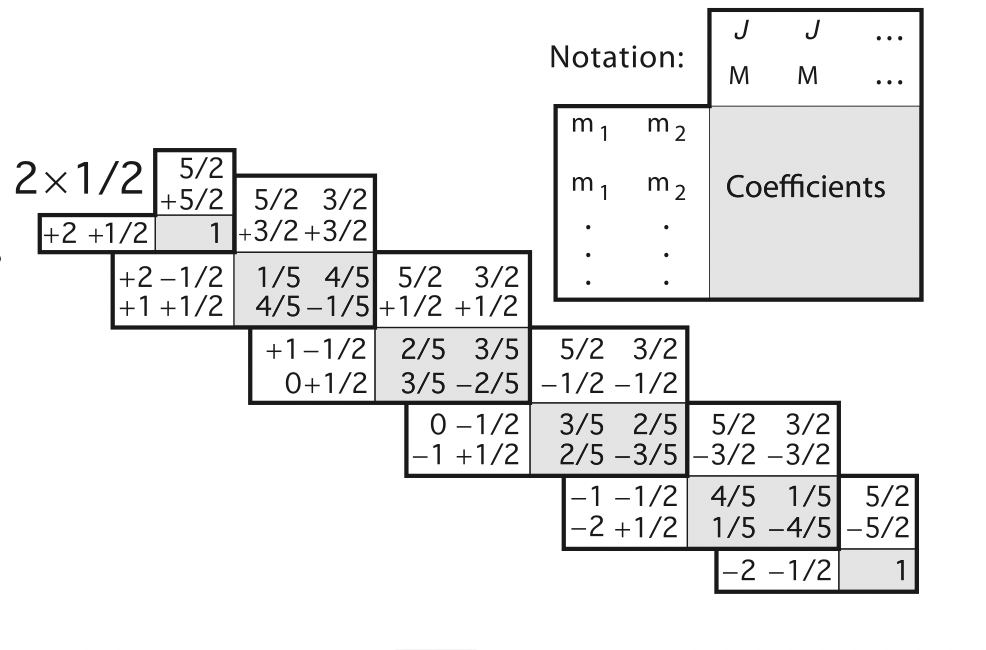
\includegraphics{../figs/clebsch-gordan-table}
    \caption{Tavola dei coefficienti di Clebsch-Gordan per composizioni di stati con
        $J_1=2$ e $ J_2 = 1/2$. \\
        Un simbolo di radice quadrata è da intendersi applicato ad ogni coefficiente.}
    \label{fig:clebsch-gordan-table}
\end{figure}

In relazione alla (\ref{eq:clebsch-gordan-def}) dalla tavola otteniamo le seguenti composizioni
\begin{gather*}
    \mathlarger{\psi}_{2,2}\mathlarger{\psi}_{\frac{1}{2}, \frac{1}{2}} = \sqrt{ 1 } \mathlarger{\psi}_{\frac{5}{2}, \frac{5}{2}}\\
    \mathlarger{\psi}_{2,2}\mathlarger{\psi}_{\frac{1}{2},- \frac{1}{2}} = \sqrt{ \frac{1}{5} } \mathlarger{\psi}_{\frac{5}{2}, \frac{3}{2}} + \sqrt{ \frac{4}{5} } \mathlarger{\psi}_{\frac{3}{2}, \frac{3}{2}}
\end{gather*}
vediamo allora che componendo gli stati di momento angolare definito (2,2) e (1/2,-1/2) otteniamo uno stato di momento angolare complessivo indefinito, sovrapposizione degli stati (5/2,3/2) e (3/2,3/2) con certi pesi.
Secondo le regole generali della meccanica quantistica ciò significa che, qualora facessimo una misura di momento angolare dell’intero sistema,
lo stato cambierebbe repentinamente ‘collassando’ su uno dei due stati componenti e precisamente avremmo probabilità 1/5 di
farlo ‘collassare’ nello stato (5/2,3/2) e probabilità 4/5 di farlo ‘collassare’ nello stato (3/2,3/2). \\
In relazione alle (\ref{eq:inverse-clebsch-gordan}) dalla tavola otteniamo anche
\[
\mathlarger{\psi}_{\frac{5}{2}, \frac{1}{2}} = \sqrt{ \frac{2}{5} } \mathlarger{\psi}_{2,1}\mathlarger{\psi}_{\frac{1}{2}, - \frac{1}{2}} + \sqrt{ \frac{3}{5} } \mathlarger{\psi}_{2,0}\mathlarger{\psi}_{\frac{1}{2}, \frac{1}{2}}
\]
vediamo allora che, dati due sottosistemi con numeri quantici del momento angolare $j_{1}=1, j_{2}=\frac{1}{2}$, lo stato di momento angolare complessivo definito (5/2,1/2) è una sovrapposizione degli stati (2,1)$\times$(1/2,-1/2) e (2,0)$\times$(1/2,1/2) con certi pesi.
Secondo le regole generali della meccanica quantistica ciò significa che, qualora facessimo una misura di momento angolare dei due sottosistemi avremmo probabilità 2/5 di farli ‘collassare’ negli stati (2,1) e (1/2,-1/2) e probabilità 3/5 di farli collassare negli stati (2,0) e (1/2,1/2).
\bigskip

Un esempio di tavola di Coefficienti di Clebsch-Gordan si trova al seguente URL:
\begin{center}
    \url{https://pdg.lbl.gov/2013/reviews/rpp2013-rev-clebsch-gordan-coefs.pdf}
\end{center}

\section{Stati quantomeccanici di due particelle identiche}\label{sec:particelle-identiche}
Lo studio dei sistemi quantomeccanici formati da particelle identiche conduce a nuove sorprendenti proprietà che non trovano alcuna analogia nella fisica classica. Entreremo nel vivo di questo affascinante problema con un esempio.
\bigskip

Immaginiamo che, in ambito macroscopico e dunque soggetti alle \emph{leggi della fisica classica}, in una certa porzione di spazio si muovano due piccole sferette, illuminate ad intervalli di tempo regolari da una luce stroboscopica (vedi Figura~\ref{fig:identical-part1}).
Il lampo luminoso al tempo $t'$ mostrerà le due sferette nelle posizioni $r_{1}'$ ed $r_{2}'$, quello al tempo $t''$ in $r_{1}''$ ed $r_{2}''$.
\begin{marginfigure}
    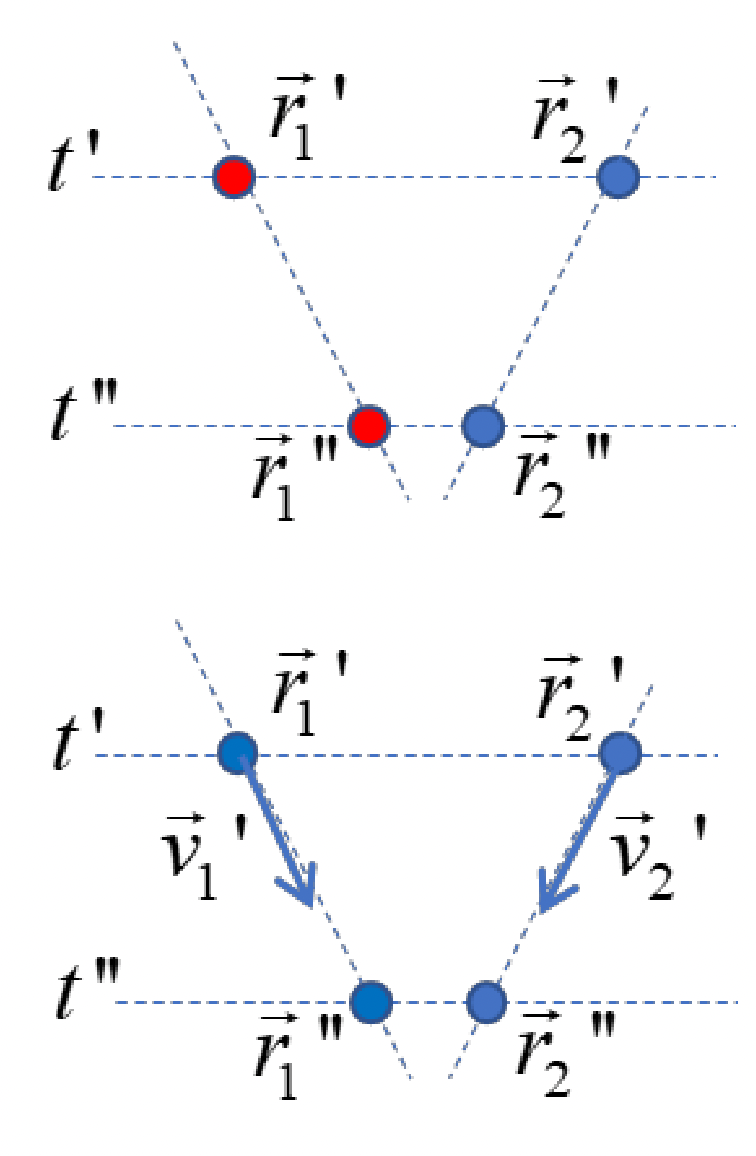
\includegraphics{figs/identical-part1}
    \caption{Set of two particles in two different classical states.}
    \label{fig:identical-part1}
\end{marginfigure}
Con tutta evidenza, se le due sferette sono \emph{diverse} non esiste alcun problema nell’associare ad ogni posizione la propria sferetta nei due istanti di tempo. Si dice allora che \emph{in meccanica classica due particelle diverse sono sempre distinguibili}.

Cio vale anche nel caso in cui le due sferette siano \emph{identiche}. Infatti, se da un lato è vero che l’identità genera una ambiguità poiché non sapremmo dire se la sferetta in $r_{1}''$($r_{2}''$) al tempo $t''$ fosse quella che al tempo $t'$ si trovava in $r_{1}'$ o $r_{2}'$; dall’altro si tratta di un’ambiguità non essenziale che può essere superata qualora note al tempo $t'$ non solo le posizioni delle sferette, ma anche le loro velocità $v_{1}'$ e $v_{2}'$, dato che al tempo $t''$ ciascuna sferetta dovrà trovarsi non troppo lontano dalla direzione della propria velocità al tempo $t'$. Poiché in ambito macroscopico non ci sono limitazioni nel conoscere in ogni istante di tempo le posizioni e le velocità delle particelle in gioco, concludiamo – come anticipato - che \textbf{nella meccanica classica sia le particelle diverse che quelle identiche sono sempre distinguibili}.
\bigskip

Cosa accade nell’ambito microscopico governato dalla meccanica quantistica? E’ semplice rendersi conto che nel caso di \emph{particelle diverse} una ipotetica misura di massa, carica o di una qualunque variabile interna capace di determinarne l’identità ci permetterà di assegnare ad ogni particella la propria posizione, in ogni istante di tempo senza ambiguità. Analogamente al caso macroscopico concludiamo allora che \textbf{nella meccanica quantistica due particelle diverse sono sempre distinguibili}.

Assai diverso è il caso in cui si abbia a che fare con \emph{particelle identiche}. Infatti - a differenza di ciò che accade nella meccanica classica – uno stato quantomeccanico non può possedere in ogni istate di tempo sia posizioni che velocità definite (principio di indeterminazione).
\begin{marginfigure}
    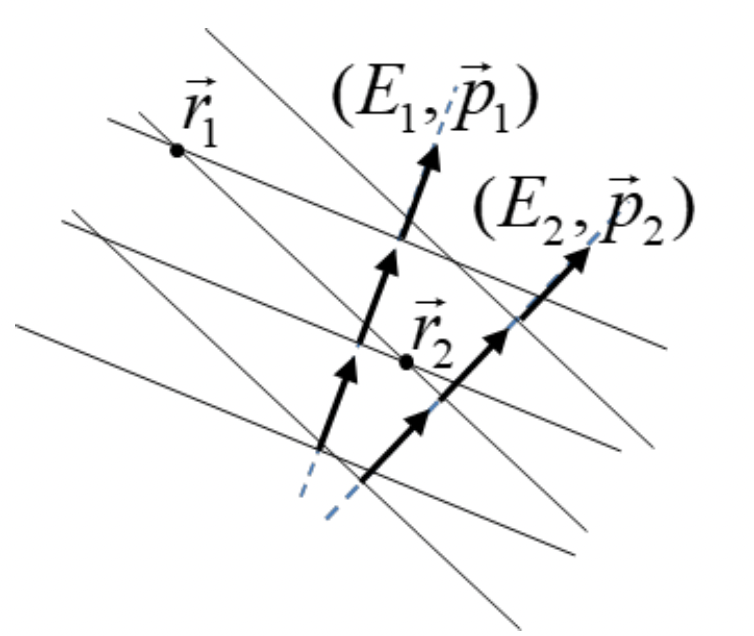
\includegraphics{figs/identical-part2}
    \caption{Set of two particles in two different quantum states.}
    \label{fig:identical-part2}
\end{marginfigure}
Se al tempo $t'$ sono definite le posizioni $r_{1}'$ e $r_{2}'$ delle particelle identiche, risulteranno allora indefinite le loro velocità $v_{1}'$ e $v_{2}'$, pregiudicando la possibilità di attribuirgli univocamente una posizione al tempo $t''$. Se, invece, al tempo $t'$ sono definite le velocità $v_{1}'$ e $v_{2}'$ delle particelle identiche (ovvero sono descritte da onde piane progressive), risulteranno allora indefinite le loro posizioni $r_{1}'$ e $r_{2}'$ che in nessun istante di tempo potranno essere univocamente assegnate alle particelle (vedi Figura~\ref{fig:identical-part2}). Giungiamo allora a concludere che \textbf{nella meccanica quantistica due particelle identiche sono sempre indistinguibili}.

Quest’ultimo caso può guidarci alla \emph{costruzione della funzione d’onda del sistema quantomeccanico di due particelle identiche}.
Per cominciare immaginiamo che il volume spaziale (vedi figura~\ref{fig:identical-part2}) sia occupato dalle onde di De Broglie piane e progressive delle due particelle che ipotizziamo abbiano energia e quantità di moto $(E_{1},\mathbf{p}_{1})$ e $(E_{1},\mathbf{p}_{1})$. Una misura di posizione eseguita sul sistema osserverà allora le due particelle in due posizioni che indichiamo con $r_{1}$ ed $r_{2}$. Dato che le funzioni d’onda delle due particelle occupano l’intero volume, la misura di posizione potrà avere i seguenti esiti
\begin{gather*}
    \text{esito 1:} (E_{1}, \mathbf{p}_{1}) \ \text{in} \ \mathbf{r}_{1} \ \text{e} \ (E_{2}, \mathbf{p}_{2}) \ \text{in} \ \mathbf{r}_{2}\\
    \text{esito 2:} (E_{2}, \mathbf{p}_{2}) \ \text{in} \ \mathbf{r}_{1} \ \text{e} \ (E_{1}, \mathbf{p}_{1}) \ \text{in} \ \mathbf{r}_{2}
\end{gather*}
Indicate allora con la seguente notazione le funzioni d’onda delle due particelle
\begin{gather*}
    \psi_{E_{1},\mathbf{{p}_{1}}}(\mathbf{{r}},t) = A_{E_{1},\mathbf{}{p}_{1}}e^{ \frac{i}{\hbar} (\mathbf{{p}}_{1} \cdot \mathbf{{r}}-E_{1}t)}\\
    \psi_{E_{2},\mathbf{{p}_{2}}}(\mathbf{{r}},t) = A_{E_{1},\mathbf{}{p}_{1}}e^{ \frac{i}{\hbar} (\mathbf{{p}}_{2} \cdot \mathbf{{r}}-E_{2}t)}
\end{gather*}
l’esito 1 avrà densità di probabilità
\[
\propto | \psi_{E_{1},\mathbf{p}_{1}}(\mathbf{r}_{1},t)|^{2} | \psi_{E_{2},\mathbf{p}_{2}}(\mathbf{r}_{2},t)|^{2}
\]
e l’esito 2 densità di probabilità
\[
\propto | \psi_{E_{2},\mathbf{p}_{2}}(\mathbf{r}_{1},t)|^{2} | \psi_{E_{1},\mathbf{p}_{1}}(\mathbf{r}_{2},t)|^{2}
\]
In accordo con i principi generali della meccanica quantistica ciò significa che la funzione d’onda del sistema delle due particelle deve essere data dalla seguente sovrapposizione coerente
\begin{equation}
    \psi_{sis} = \alpha \, \psi_{E_{1},\bm{p}_{1}}(\textcolor{cyan}{\bm{r_1}},t) \psi_{E_{2},\bm{p}_{2}}(\textcolor{orange}{\bm{r_2}},t) +
    \beta \, \psi_{E_{2},\bm{p}_{2}}(\textcolor{cyan}{\bm{r_1}},t) \psi_{E_{1},\bm{p}_{1}}(\textcolor{orange}{\bm{r_2}},t)
    \label{eq:total-system-wave-function-identical-particles}
\end{equation}
governata da due coefficienti complessi $\alpha$ e $\beta$ sui quali, per ora, non sappiamo dire di più, fatto che genera una ambiguità nota con il nome di \textbf{degenerazione di scambio}.
\bigskip

Si noti che ancora non abbiamo imposto che le particelle del sistema siano identiche.
Vedremo che sarà proprio questo requisito che rimuoverà la degenerazione di scambio.
Il modo per esprimere formalmente in meccanica quantistica l’identità delle particelle o \textbf{principio di
indistinguibilità delle particelle} è quello di richiedere che \emph{a seguito dello scambio delle particelle tutte le
grandezze fisiche osservabili rimangano immutate}.
Dato che \textbf{in meccanica quantistica ciò che è osservabile non è la funzione d’onda ma il suo modulo quadrato}, dobbiamo allora  richiedere che
%
%Lo studio dei sistemi quantomeccanici formati da particelle identiche conduce a nuove
%sorprendenti proprietà che non trovano alcuna analogia nella fisica
%classica.
%Vediamo un esempio.
%
%Immaginiamo di essere in ambito macroscopico e quindi soggetti alle
%leggi della \emph{fisica classica}.
%
%Immaginiamo poi che, in una certa porzione di spazio, si muovano due
%piccole sferette, e che tale spazio sia illuminato ad intervalli di
%tempo regolari da una luce stroboscopica (vedi Figura~\ref{fig:identical-part1}).
%Il lampo luminoso al tempo
%\(t'\) mostrerà le due sferette nelle posizioni \(r_{1}'\) e \(r_{2}'\)
%e quello al tempo \(t''\) in \(r_{1}''\) e \(r_{2}''\).
%\begin{marginfigure}
%    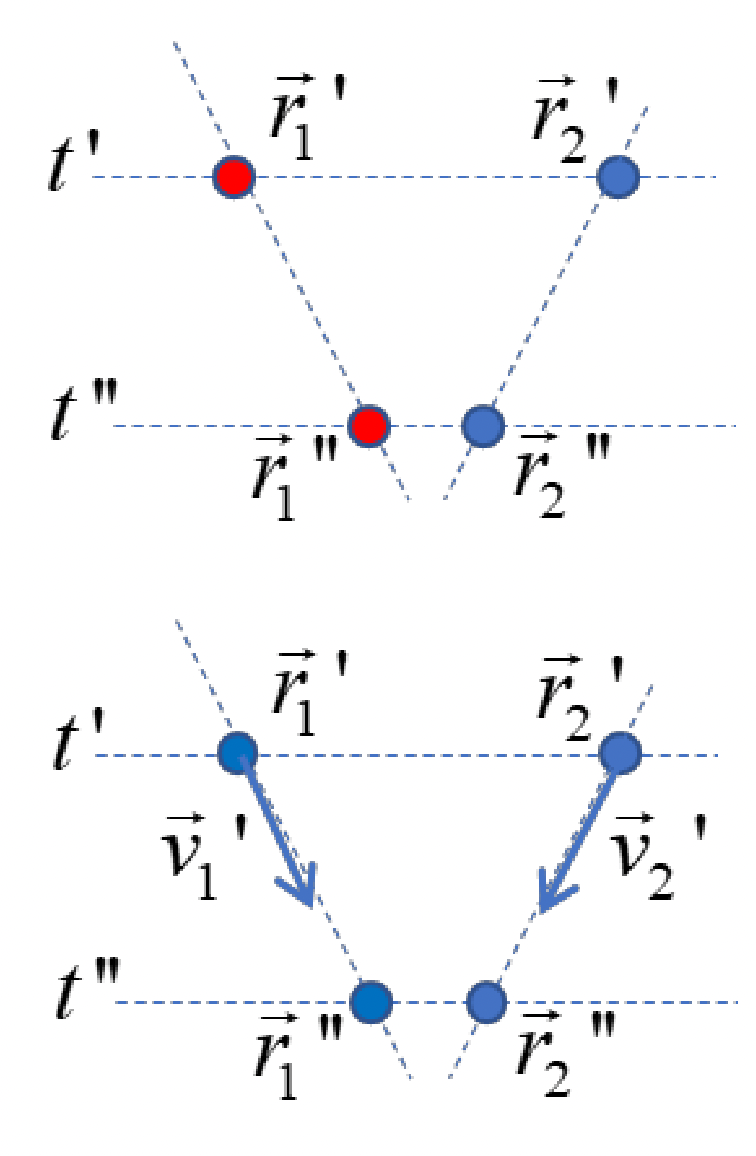
\includegraphics{figs/identical-part1}
%    \caption{Set of two particles in two different classical states.}
%    \label{fig:identical-part1}
%\end{marginfigure}
%Con tutta evidenza, se le due sferette sono diverse non esiste alcun problema
%nell'associare alle posizioni osservate, in ogni dato istante di tempo,
%la specifica sferetta.
%Si dice allora che in meccanica classica due
%particelle diverse sono sempre distinguibili.
%
%Diverso sembra il caso in cui le due sferette siano identiche.
%Infatti,
%non sapremmo dire se la sferetta nella posizione \(r_{1}''(r_{2}'')\) al
%tempo \(t''\) sia quella che al tempo \(t'\) si trovava in \(r_{1}'\) o
%quella che si trovava in \(r_{2}'\).
%L'identità delle sferette ci ha
%condotti dunque alla impossibilità di associare con certezza le
%posizioni alle particelle.
%L'ambiguità, però, non è essenziale poichè
%può essere superata qualora al tempo t' siano note, non solo le
%posizioni delle sferette, ma anche le loro velocità \(v_1'\) e \(v_2'\).
%Infatti, al tempo \(t''\) ciascuna sferetta dovrà trovarsi non troppo
%lontano dalla direzione della propria velocità al tempo \(t'\) (se
%l'istante \(t''\) non è troppo lontano da \(t'\)).
%Concludiamo allora
%che, se in un istante di tempo le posizioni e le velocità di due
%sferette identiche sono note con sufficiente precisione, \emph{sarà sempre
%possibile determinare la loro posizione in ogni istante di tempo
%successivo}.
%
%Poiché nella meccanica classica non ci sono limitazioni nel conoscere in
%ogni istante di tempo le posizioni e le velocità delle particelle in
%gioco, concludiamo che \textbf{nella fisica classica sia le particelle
%diverse che quelle identiche sono sempre distinguibili}.
%\bigskip
%
%Cosa accade in meccanica quantistica?
%E' semplice rendersi conto che nel
%caso di particelle diverse una ipotetica misura di massa, carica o di
%una qualunque variabile interna capace di determinarne l'identità sarà
%in grado di dirci senza ambiguità quale posizione occupi ciascuna delle
%due particelle.
%Dunque, analogamente al caso della meccanica classica,
%giungiamo quindi ad affermare che \emph{nella meccanica quantistica due
%particelle diverse sono sempre distinguibili}.
%
%Ben diverso è il caso in cui le particelle siano identiche.
%Infatti - a
%differenza di ciò che accade in meccanica classica -- uno stato
%quantomeccanico non può possedere in ogni istante di tempo sia posizioni
%definite che velocità definite (principio di indeterminazione).
%
%Se ad
%esempio al tempo \(t'\) sono definite le posizioni \(r_{1}'\) e
%\(r_{2}'\) delle due particelle identiche, risulteranno allora
%indefinite le corrispondenti velocità \(v_{1}'\) e \(v_{2}'\)
%pregiudicando dunque la possibilità di attribuire univocamente una
%posizione a ciascuna di esse al tempo t'\,.
%Analogamente, se al tempo
%t' sono definite le velocità \(v_{1}'\) e \(v_{2}'\) delle due
%particelle identiche (e dunque le quantità di moto), risulteranno allora
%indefinite le loro posizioni che non potranno essere univocamente
%assegnate alle particelle stesse.
%
%%Giungiamo allora a concludere che \textbf{nella meccanica quantistica
%%due particelle identiche sono sempre indistinguibili}.
%%Tale fatto può
%%essere visto in modo ancor più diretto attraverso il seguente esempio.
%%Immaginiamo di avere due particelle microscopiche identiche che
%%si trovino in stati quantomeccanici diversi, ad esempio di quantità di
%%moto ed energia (\(E_1, p_1\)) ed (\(E_2, p_2\)) descritte da due onde
%%piane di De Broglie (vedi figura~\ref{fig:identical-part2}).
%
%%Con tutta evidenza due misure di posizione potranno trovare la
%%particella (\(E_{1},p_{1}\)) nella posizione \(r_{1}\) e la particella
%%(\(E_{2},p_{2}\)) nella posizione \(r_{2}\), oppure la particella
%%(\(E_{2}, p_{2}\)) nella posizione \(r_{1}\) e la particella
%%(\(E_{1}, p_{1}\)) nella posizione \(r_{2}\), dando quindi luogo alla
%%ambiguità discussa.
%%\bigskip
%%
%%L'esempio può guidarci anche alla costruzione della funzione d'onda del
%%sistema quantomeccanico delle due particelle identiche.\\
%%Per cominciare consideriamo due particelle identiche poste in regioni di
%%spazio differenti ovvero mutuamente isolate (ad esempio ponendole in
%%contenitori diversi).
%%La densità di probabilità di osservare la
%%particella (\(E_{1},p_{1}\)) nella posizione \(r_{1}\) e la particella
%%(\(E_{2},p_{2}\)) nella posizione \(r_{2}\) è data allora dal modulo
%%quadrato della seguente funzione d'onda
%%\begin{equation}
%%    \psi_{E_{1},\bm{p}_{1}}(\textcolor{cyan}{\bm{r_1}},t) \psi_{E_{2},\bm{p}_{2}}(\textcolor{orange}{\bm{r_2}},t)
%%    \label{eq:identical-part-product-wave-functions}
%%\end{equation}
%%dove i termini a prodotto sono le funzioni d'onda delle singole
%%particelle \begin{gather*}
%%               \psi_{E_{1},\bm{p}_{1}}(\textcolor{cyan}{\bm{r_1}},t) = A_{E_{1},\bm{p}_{1}}e^{ \frac{i}{\hbar} (\bm{p}_{1} \cdot \textcolor{cyan}{\bm{r_1}}-E_{1}t)}\\
%%               \psi_{E_{2},\bm{p}_{2}}(\textcolor{orange}{\bm{r_2}},t) = A_{E_{2},\bm{p}_{2}}e^{ \frac{i}{\hbar} (\bm{p}_{2} \cdot \textcolor{orange}{\bm{r_2}}-E_{2}t)}
%%\end{gather*}
%%Se ora rimuoviamo la condizione di isolamento, costruendo un unico
%%sistema fisico formato da due particelle identiche poste nella stessa
%%regione di spazio (ad esempio mettendole entrambe nello stesso
%%contenitore) ci rendiamo subito conto che la funzione d'onda (\ref{eq:identical-part-product-wave-functions})
%%non descrive lo stato quantomeccanico in modo completo.
%%Infatti - come
%%osservato in precedenza - è anche possibile che una misura di posizione
%%sul sistema trovi la particella (\(E_{2},p_{2}\)) in \(r_{1}\) e la
%%particella (\(E_{1},p_{1}\)) in \(r_{2}\), un esito evidentemente non
%%descritto dalla (\ref{eq:identical-part-product-wave-functions}).
%%Tale esito è invece descritto dalla seguente funzione d'onda
%%\begin{equation}
%%    \psi_{E_{2},\bm{p}_{2}}(\bm{r}_{1},t) \psi_{E_{1},\bm{p}_{1}}(\bm{r}_{2},t)
%%    \label{eq:identical-part-product-wave-functions-2}
%%\end{equation} dove i termini a prodotto sono dati dalle funzioni d'onda
%%delle singole particelle
%%\begin{gather*}
%%    \psi_{E_{1},\bm{p}_{1}}(\textcolor{orange}{\bm{r_2}},t) = A_{E_{1},\bm{p}_{1}}e^{ \frac{i}{\hbar} (\bm{p}_{1} \cdot \textcolor{orange}{\bm{r_2}}-E_{1}t)}\\
%%    \psi_{E_{2},\bm{p}_{2}}(\textcolor{cyan}{\bm{r_1}},t) = A_{E_{2},\bm{p}_{2}}e^{ \frac{i}{\hbar} (\bm{p}_{2} \cdot \textcolor{cyan}{\bm{r_1}}-E_{2}t)}
%%\end{gather*}
%%Ora, dato che il sistema di due particelle identiche può dare luogo
%%ad entrambi gli esiti (\ref{eq:identical-part-product-wave-functions}) e (\ref{eq:identical-part-product-wave-functions-2}),
%%tali esiti - in accordo con
%%i principi generali della meccanica quantistica - dovranno essere
%%sommati coerentemente.
%%In assenza di ulteriori prescrizioni, non potremo
%%che introdurre due generici coefficienti complessi ottenendo uno stato
%%che - pur soddisfacendo i requisiti richiesti - contiene due
%%coefficienti arbitrari
%%\[
%%    \psi_{sis} = \alpha \, \psi_{E_{1},\bm{p}_{1}}(\bm{r}_{1},t) \psi_{E_{2},\bm{p}_{2}}(\bm{r}_{2},t) +
%%    \beta \, \psi_{E_{2},\bm{p}_{2}}(\bm{r}_{1},t) \psi_{E_{1},\bm{p}_{1}}(\bm{r}_{2},t)
%%\]
%%una ambiguità nota con il nome di \textbf{degenerazione di scambio}.
%%\bigskip
%%
%%Tale degenerazione può essere rimossa richiedendo che sia soddisfatto il \textbf{principio di indistinguibilità delle particelle
%%identiche} valido in meccanica quantistica.
%%Tale principio può essere espresso in forma operativa richiedendo che a seguito di uno scambio delle posizioni delle particelle identiche tutte le grandezze fisiche osservabili rimangano immutate.
%%Ricordando che in meccanica quantistica ciò che è osservabile non è la funzione d’onda ma il suo modulo quadrato, dobbiamo allora a richiedere che
\begin{equation}
    |\mathlarger{\psi}_{sist}^{scambio}|^2 = |\mathlarger{\psi}_{sist}|^2
    \label{eq:indistinguishable-particles-principle}
\end{equation}
un fatto che non esclude che la funzione d’onda, invece, possa modificarsi a seguito dello scambio.
\bigskip

A questo punto non dobbiamo far altro che costruire $ \mathlarger{\psi}^{scambio}_{sist}$
a partire da (\ref{eq:total-system-wave-function-identical-particles}) ed imporre la validità di (\ref{eq:indistinguishable-particles-principle})\sidenote
{
Introduciamo la notazione seguente:
\begin{gather*}
    \psi_1 \equiv \psi_{E_1,\bm{p}_1} \\
    \psi_2 \equiv \psi_{E_2,\bm{p}_2}
\end{gather*}
}:
\[
    |\alpha\, \psi_2(\bm{r}_1)\,\psi_1(\bm{r}_2) + \beta\, \psi_1(\bm{r}_1)\,\psi_2(\bm{r}_2)|^2 =
    |\alpha\, \psi_1(\bm{r}_1)\,\psi_2(\bm{r}_2) + \beta\, \psi_2(\bm{r}_1)\,\psi_1(\bm{r}_2)|^2
\]
da cui si ottengono le condizioni seguenti
\begin{align*}
    &|\beta|^{2} = |\alpha|^{2} \qquad \alpha \bar{\beta} = \beta \bar{\alpha}  \\
    &\alpha = ae^{ ia' } \quad \ \  \quad  \beta = b e^{ ib' }  \\
    &b^{2} = a^{2} \qquad \quad \, ab e^{ i(a'-b') } = abe^{ -i(a'-b') } \\
    &b = \pm a \qquad \quad a'-b'=0 \\
    &\alpha = a e^{ ia' } \qquad \ \beta = \pm ae^{ ia' }
\end{align*}
Dato che il fattore $ e^{ia}$ può essere raccolto a fattor comune e riassorbito come
coefficiente di normalizzazione, otteniamo la seguente espressione della \textbf{funzione d’onda del sistema quantomeccanico
di due particelle identiche}
\begin{equation}
    \psi_{sist} = \psi_{E_1, \bm{p_1}} (\bm{r_1}, t) \, \psi_{E_2, \bm{p_2}} (\bm{r_2}, t) \pm \psi_{E_1, \bm{p_1}} (\bm{r_2}, t) \, \psi_{E_2, \bm{p_2}} (\bm{r_1}, t).
    \label{eq:identical-particles-wave-function}
\end{equation}
Giungiamo così alla conclusione che \textbf{un sistema quantomeccanico di due particelle identiche è descritto da una funzione
d’onda simmetrica o antisimmetrica rispetto allo scambio delle particelle stesse}.

Una prima sorprendente conclusione di ordine generale riguarda il fatto che ci sono due diversi modi di costruire la
funzione d’onda di un sistema di due o più particelle microscopiche identiche, modi che permettono di separare
le particelle microscopiche in due grandi famiglie.
La famiglia delle particelle che richiedono uno stato quantomeccanico simmetrico rispetto allo scambio
(opzione con segno positivo) e la famiglia delle particelle che richiedono uno stato quantomeccanico antisimmetrico
rispetto allo scambio (opzione con segno negativo), in sostanza una \textbf{ delle particelle basata sulle loro proprietà
collettive}.
Abbiamo:
\begin{itemize}
    \item \textbf{particelle di Bose-Einstein} o \textbf{bosoni}, che richiedono simmetria.
    Sono bosoni i mediatori delle forze elementari, detti \textit{di gauge};
    \item \textbf{particelle di Fermi-Dirac} o \textbf{fermioni}, che richiedono antisimmetria e per loro vale il
    \textbf{principio di esclusione di Pauli}:
    due fermioni non possono disporsi nello stesso stato quantomeccanico poiché ciò annullerebbe la funzione d'onda del sistema
    (\ref{eq:identical-particles-wave-function}).
    Le particelle atomiche (come ogni quark e leptone) sono fermioni.
\end{itemize}
Vi è inoltre uno strettissimo legame tra spin e proprietà collettive di simmetria, dato dal fondamentale \textbf{teorema spin-statistica}:
particelle identiche di spin \textit{intero} sono \textit{bosoni}, mentre di spin \textit{semi-intero} sono \textit{fermioni}.
Nel vuoto, a differenza che nei mezzi materiali e nel caso di eccitazioni collettive, le particelle microscopiche si
comportano sempre in accordo a tale teorema e non vi sono situazioni di simmetria mista.